% est�mme ihme "underfull \hbox (badness 10000)" -varoitukset (ei hajua mist� tulevat)
\hbadness=10000

% makrot dokumentoinnin generoimiseksi

% Macros for generating design documents and .java files

% MACROS FOR CLASS DOCUMENTATION
\newcommand{\getClass}[0]{}
\newcommand{\beginClass}[1] {
	\subsubsection{#1}
	
	\renewcommand{\getClass}[0]{#1}
	\label{class:#1}
	
	\begin{hyphenrules}{nohyphenation}
	\begin{tabular}{p{3cm}p{11cm}}
}
\newcommand{\classComment}[1] {
	\multicolumn{2}{p{14cm}} {
		#1
	}\\
}
\newcommand{\classPackage}[1] {
	\textbf{Package} & #1 \\
}
\newcommand{\classDeclaration}[1] {
	\textbf{Declaration} & #1 \\
}
\newcommand{\classExtends}[1] {
	\textbf{Extends} & #1 \\
}
\newcommand{\classImplements}[1] {
	\textbf{Implements} & #1 \\
}
\newcommand{\classCreatedBy}[1] {
	\textbf{Created by} & #1 (\ref{class:#1}) \\
}
\newcommand{\classUses}[1] {
	\stepcounter{classUsesCounter}
	\textbf{Uses \arabic{classUsesCounter}} & #1 (\ref{class:#1}) \\
}
\newcommand{\classSubclass}[1] {
	\stepcounter{classSubclassCounter}
	\textbf{Subclass \arabic{classSubclassCounter}} & #1 (\ref{class:#1}) \\
}
\newcommand{\classPatterns}[1] {
	\textbf{Design patterns} & #1 \\
}
\newcommand{\classEvent}[2] {
	\stepcounter{classEventCounter}
	\textbf{Event \Alph{classEventCounter}} & \textit{#1} - #2 \\
}
\newcommand{\closeClass}[0] {
	\end{tabular}\\
	\end{hyphenrules}
	
	\setcounter{classUsesCounter}{0}
	\setcounter{classSubclassCounter}{0}
	\setcounter{classEventCounter}{0}
	
	\renewcommand{\isFirstField}[0]{ \large\textbf{Fields of \getClass}\normalsize }
	\renewcommand{\isFirstMethod}[0]{ \large\textbf{Methods of \getClass}\normalsize }
}
\newcounter{classUsesCounter}
\newcounter{classSubclassCounter}
\newcounter{classEventCounter}
\newcommand{\isFirstField}[0]{}
\newcommand{\isFirstMethod}[0]{}


% MACROS FOR CLASS TABLE OF CONTENTS
\newcommand{\beginToc}[0] {
	\begin{hyphenrules}{nohyphenation}
	%\begin{tabular*}{14cm}{lr}
	\begin{tabular*}{14cm}{@{\extracolsep{\fill}}lr}
	\textbf{Method} & \textbf{Page} \\
}
\newcommand{\tocMethod}[1] {
	#1 & \pageref{method:\getClass.#1} \\
}
\newcommand{\closeToc}[0] {
	\end{tabular*}\\
	\end{hyphenrules}
}


% MACROS FOR FIELD DOCUMENTATION
\newcommand{\getField}[0]{}
\newcommand{\beginField}[1] {
	\isFirstField
	\renewcommand{\isFirstField}[0]{}
	
	\renewcommand{\getField}[0]{#1}
	\label{field:\getClass.#1}
	
	\begin{hyphenrules}{nohyphenation}
	\begin{tabular}{p{3cm}p{11cm}}
}
\newcommand{\fieldDeclaration}[1] {
	\multicolumn{2}{p{14cm}} {
		\hspace{-0.32cm}
%		\large{\textsf{#1}}
		\textsf{#1}
	}\\
}
\newcommand{\fieldValue}[1] {
	\textbf{Default value} & #1 \\
}
\newcommand{\fieldComment}[1] {
	\multicolumn{2}{p{14cm}} {
		#1
	}\\
}
\newcommand{\closeField}[0] {
	\end{tabular}\\
	\end{hyphenrules}
}


% MACROS FOR METHOD DOCUMENTATION
\newcommand{\getMethod}[0]{}
\newcommand{\beginMethod}[1] {
	\isFirstMethod
	\renewcommand{\isFirstMethod}[0]{}
	
	\renewcommand{\getMethod}[0]{#1}
	\label{method:\getClass.#1}
	
	\begin{hyphenrules}{nohyphenation}
	\begin{tabular}{p{3cm}p{11cm}}
}
\newcommand{\methodDeclaration}[1] {
	\multicolumn{2}{p{14cm}} {
		\hspace{-0.32cm}
%		\large{\textsf{#1}}
		\textsf{#1}
	}\\
}
\newcommand{\methodComment}[1] {
	\multicolumn{2}{p{14cm}} {
		#1
	}\\
}
\newcommand{\methodParam}[2] {
	\stepcounter{methodParamCounter}
	\textbf{Parameter \arabic{methodParamCounter}} & \textit{#1} - #2 \\
}
\newcommand{\methodReturn}[1] {
	\textbf{Returns} & #1 \\
}
\newcommand{\methodThrows}[2] {
	\textbf{Throws} & \textit{#1} - #2 \\
}
\newcommand{\closeMethod}[0] {
	\end{tabular}\\
	\end{hyphenrules}
	\setcounter{methodParamCounter}{0}
}
\newcounter{methodParamCounter}



% nopsa pikkuluokkakaavioiden lis�ysmakro
% pois figuren sis�lt� niin kuvat tulee minne pit��kin, ilman kuvateksti� ja kuvanumerointia tosin
\newcommand{\insertdia}[1] {
	% \begin{figure}[h]
	\begin{center}
	\includegraphics[scale=0.33]{dia/#1.eps}
	% \includegraphics[width=#2]{dia/#1.eps}
	% \caption{#3}
	% \label{fig:#1}
	\end{center}
	% \end{figure}
}

\section{Introduction}
\label{sec:intro}

This document describes planned architecture for the SQUID magnetometer program that will be implemented as a software engineering student project at University of Helsinki, Department of Computer Science. The clients are Lauri Pesonen with his assistants Fabio Donadini and Tomas Kohout from Department of Geophysics.

The document serves as an internal guide to the project team for aiding implementation phase, and describes the software at about level of accuracy which allows to implement the software based on this document and requirements document (version 1.1), which has user interface prototypes as appendices, and on which this document is based.

\subsection{Structure of the document}

\par Section~\ref{sec:intro} (this section) describes the meaning and structure of the document.
\par Section~\ref{sec:code} describes coding conventions used by the project group in this sowtware.
\par Section~\ref{sec:over} describes the software and architecture at high abstarction.
\par Section~\ref{sec:arch} describes planned architecture at lower abstarction, including class diagrams and a short description of each subsystem.
\par Section~\ref{sec:data} describes planned data classes.
\par Section~\ref{sec:gui} describes planned gui classes.


\section{Code conventions}
\label{sec:code}

Everybody will follow the Code Conventions for the Java Programming Language set by Sun, with the following refinements.

\begin{itemize}
\item Line length will be set to 120 characters, because we prefer coding in high resolutions.
\item If possible, set your IDE to use spaces instead of tabs (to avoid problems if somebody has set tab to 4 spaces, although it should be 8). Indentation is 4 spaces, as set by Sun.
\item Every method and non-trivial field must have Javadoc comments. Every parameter, return value and exception of methods must be mentioned (except for trivial getters and setters).
\item Every if, for and while loop must use braces \texttt{\{\}}, even when there will be only one statement in the block, as set by Sun.
\item The @author comment for every class should have the name of the person who wrote (and designed) the class. Then we will know who to ask, if there are some questions about the code.
\item Every source file is subject to automatic code reformatting by a Java IDE, in which case the reformatter must follow these code conventions.
\item TODO-comments should be set by the programmer, if there is some part that needs more work. The format is \texttt{"// TODO: comments"}
\end{itemize}

The Code Conventions are available at \\
\texttt{http://java.sun.com/docs/codeconv/}

This program will be written with Java 1.5. Every programmer should have a look at the new features that were introduced to the Java language. Especially noteworthy are Generics, Foreach-loop and Enums. The following article will explain them in a nutshell. \\
\texttt{http://java.sun.com/developer/technicalArticles/releases/j2se15/}

It is recommendable for everybody to have a quick glance at Design Patterns. Here are some useful links. \\
\texttt{http://sern.ucalgary.ca/courses/SENG/609.04/W98/notes/} \\
\texttt{http://www.dofactory.com/Patterns/Patterns.aspx}


\section{Overview of the system}
\label{sec:over}

This system has two different separete project, Ikayaki-program and Squid Emulator which is subproject. Ikayaki, as main project, has graphical user interface (see requirements-document) and interface for communicating with SQUID magnetometer (Superconducting Quantum Interference Device) to measusure magnetization of minerals and rocks. Squid Emulator is vital for testing Ikayaki and it will be simple command-line program which emulates only data flow with random data and communication.

Software is split in two main parts in this document. Data section includes files needed for project-management, data flow in software and interface to control SQUID-system. There is also Settings for whole system and a subproject squid emulator. User Interface section documents all graphical interface classes, nothing more. There will be no graphical user interface for squid emulator.


\section{Architecture description}
\label{sec:arch}

Here we describe each subsystem shortly, and present a class diagram of each, as well as the whole system divided roughly into data and gui parts.

Note that the structure of this section is exactly the same as sections \ref{sec:data}-\ref{sec:gui}, but with only first two sectioning levels.


\subsection{Data classes and methods}

\begin{figure}
\begin{center}
\hspace{-1cm}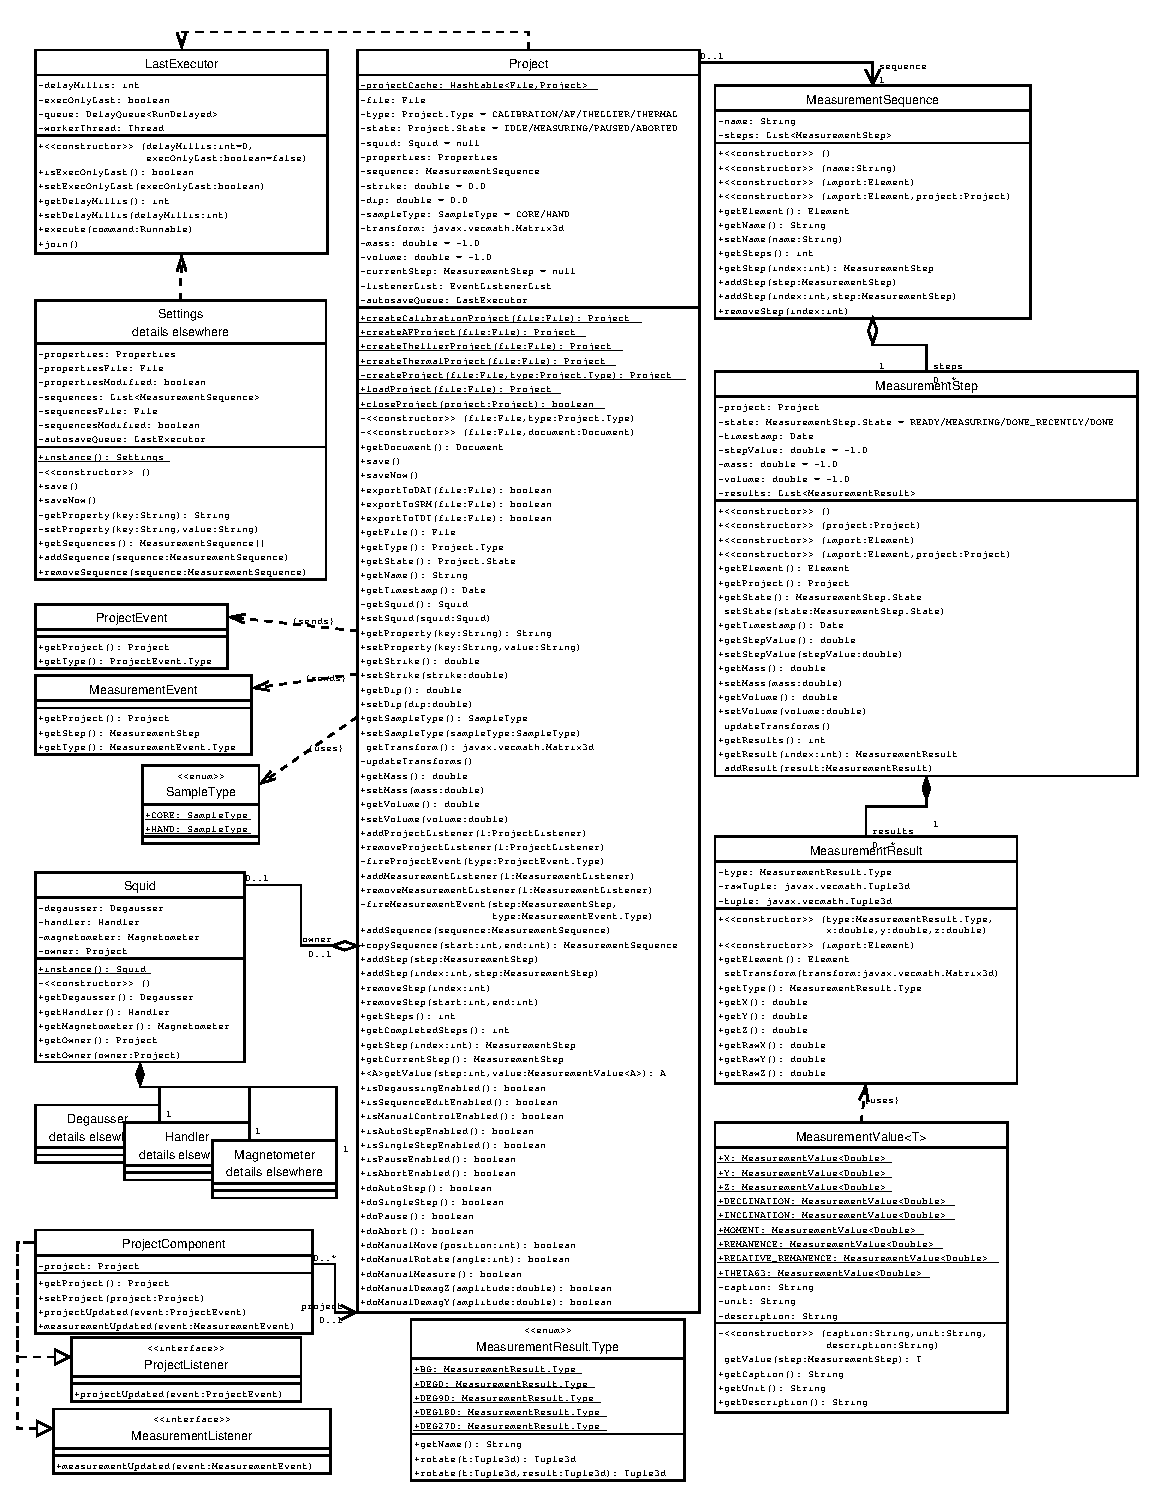
\includegraphics[width=17cm]{dia/core.eps}
\caption{Squid class diagram: data classes}
\label{fig:core}
\end{center}
\end{figure}

Class diagram of data classes is in Figure~\ref{fig:core}.

Data classes are in packages ikayaki, ikayaki.squid and ikayaki.util.

Package ikayaki holds generic data classes, ikayaki.squid holds classes loosely related to the squid interface, and ikayaki.util has utilities (\ref{sec:utilities}).

\subsubsection{Project data}

Responsible for holding all the measurement data and controlling the SQUID. Most of the GUI classes use the Project class. When the state of the project changes, the Project class fires ProjectEvents and MeasurementEvents to the GUI classes, which in turn will call the Project class to get the changed information.

\subsubsection{Squid interface}
\insertdia{core-squid}

Squid Interface offers the Project class an interface to safely control the SQUID magnetometer. It holds three subclasses that handle communication to to three separate parts of the SQUID (Handler, Degausser and Magnetometer).

Classes are Squid, Handler, Magnetometer, Degausser.

\subsubsection{Squid emulator}
\insertdia{core-squidemu}

This is separate from other and is used only for testing the Squid Interface that it works correctly.

\subsubsection{Serial communication}
\insertdia{core-serial}

SerialIO and classes related to it takes care of the harware layer of serial communication. Using these classes Ikayaki communicates with the Degausser, Samplehandler and Magnetometer. SerialIO represents one serial port and when it's created it reserves the port to itself. SerialProperties class includes all the configuration data for the serial port.

\subsubsection{Global settings}

Global properties that are used all around the program. The Settings class provides a global point for retrieving and modifying the properties.

\subsubsection{Utilities}
\label{sec:utilities}

Miscellaneous classes that are used nowhere in particular.


\subsection{GUI classes and methods}

\begin{figure}
\begin{center}
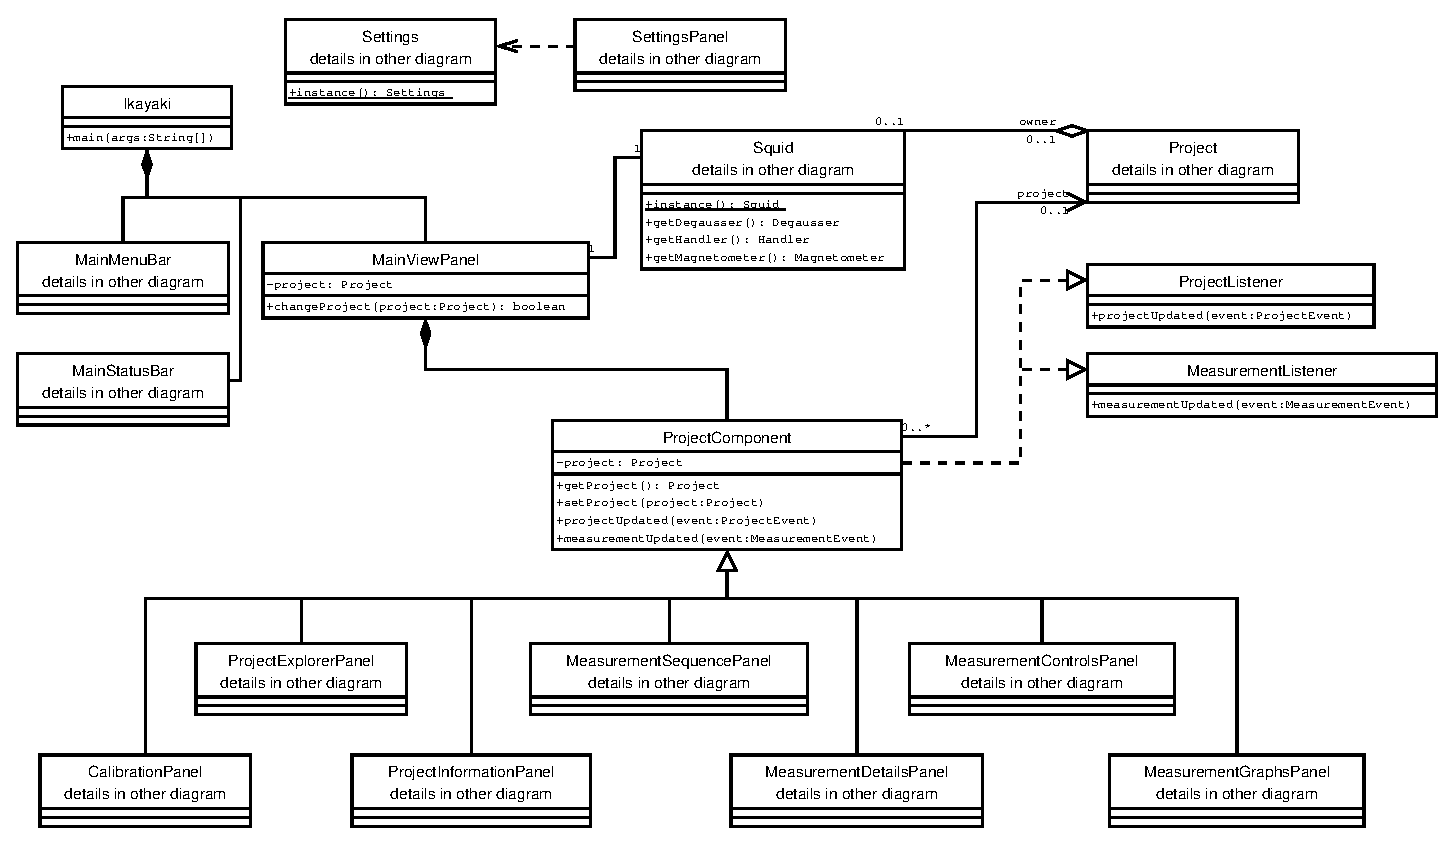
\includegraphics[angle=90,width=12cm]{dia/gui.eps}
\caption{Squid class diagram: GUI classes}
\label{fig:gui}
\end{center}
\end{figure}

Class diagram of gui classes is in Figure~\ref{fig:gui}. This section is divided into sections by gui components, each of which has one or more classes.

All gui classes are in package ikayaki.gui.

\subsubsection{Generic GUI components}

ProjectComponent, a generic gui base class which handles registering Project- and MeasurementListeners to new projects, and which every gui component subclasses.

\subsubsection{Main window}
\insertdia{gui-main}

\subsubsection{Configuration window}

\subsubsection{Project Explorer}
\insertdia{gui-explorer}

Located at middle left side of main window.

ProjectExplorerPanel handles loading existing projects and creating new ones. Shows a listing of project files in current directory, which can be changed by typing new directory into ComboBox text field, or using the browse-button and standars dir chooser dialog. ComboBox also holds directory history, and, when typing text into it's text field, automatically shows autocomplete results.

NewProjectPanel has components for creating a new project.

ProjectExplorerTable is a JTable with the project file listing, including "filename", "type" and "last modified" columns.

ProjectExplorerPopupMenu has options for exporting project files into different formats.

\subsubsection{Calibration}
\insertdia{gui-calibration}

Located at upper left corner of main window.

CalibrationPanel holds predefined "Holder noise" and "Standard sample" projects for calibration in a similar table as Project Explorer. Also has a "Calibrate" button, which executes selected calibration project, similarly to clicking "Single step" in normal projects.

\subsubsection{Project information}

\subsubsection{Sequence and measurement data}

\subsubsection{Measurement details}

\subsubsection{Measurement controls}
\insertdia{gui-mcontrols}

Located at upper right corner of main window.

MeasurementControlsPanel holds the buttons for controlling measurements, a help picture for sample inserting, radiobuttons for changing +z/-z orientation of sample, magnetometer status picture and manual controlling components.

MagnetometerStatusPanel shows an image of current magnetometer status, as in sample holder position and rotation. Image is updated according to MeasurementEvents received.

ManualControlsPanel has controls for fully manual measuring, which are enabled when no "normal" measurements are happening.

\subsubsection{Graphs}
\insertdia{gui-graphs}

Graph panels visualize the measurement data. They are located at the lower right corner in the UI. MeasurementGraphsPanel listens to MeasurementEvents to update the measurement data in plots. AbstractPlot is an abstract class which implements all the general features of graph plots. IntensityPlot and StereoPlot extend the functionality of AbstractPlot and implement their special drawing features accordingly.


\section{Data classes and methods}
\label{sec:data}

\subsection{Project data}

\beginClass{Project}
\classPackage{ikayaki}
\classDeclaration{public class Project}
\classCreatedBy{ProjectExplorerPanel}
\classUses{MeasurementSequence}
\classUses{MeasurementStep}
\classUses{MeasurementResult}
\classUses{MeasurementValue}
\classUses{Squid}
\classUses{RunQueue}
\classUses{ProjectEvent}
\classUses{MeasurementEvent}
\classComment{
	Represents a measurement project file. Project is responsible for managing and storing the data that is recieved from the magnetometer measurements. Any changes made to the project will be written to file regularly (autosave).
	
	Project is responsible for controlling the magnetometer through the SQUID API. Controlling the SQUID will be done in a private worker thread. Only one project at a time may access the SQUID.
	
	All operations are thread-safe.
}
\classPatterns{Facade}
\classEvent{On property change}{Autosaving will be invoked and the project written to file after a short delay.}
\classEvent{On measurement started/ended/paused/aborted}{ProjectEvent will be fired to all project listeners.}
\classEvent{On measurement subphase started/completed}{MeasurementEvent will be fired to all measurement listeners.}
\classEvent{On declination/inclination/volume changed}{The updated transformation matrix will be applied to all measurements and a ProjectEvent will be fired to all project listeners.}
\closeClass

\beginField{file}
\fieldDeclaration{private File file}
\fieldComment{
}
\closeField

\beginField{type}
\fieldDeclaration{private Type type}
\fieldComment{
}
\closeField

\beginField{state}
\fieldDeclaration{private State state}
\fieldValue{IDLE}
\fieldComment{
}
\closeField

\beginField{squid}
\fieldDeclaration{private Squid squid}
\fieldValue{null}
\fieldComment{
}
\closeField

\beginField{properties}
\fieldDeclaration{private Properties properties}
\fieldComment{
}
\closeField

\beginField{sequence}
\fieldDeclaration{private MeasurementSequence sequence}
\fieldComment{
}
\closeField

\beginField{strike}
\fieldDeclaration{private double strike}
\fieldValue{0.0}
\fieldComment{
}
\closeField

\beginField{dip}
\fieldDeclaration{private double dip}
\fieldValue{0.0}
\fieldComment{
}
\closeField

\beginField{transform}
\fieldDeclaration{private Matrix3d transform}
\fieldValue{new Matrix3d()}
\fieldComment{
}
\closeField

\beginField{mass}
\fieldDeclaration{private double mass}
\fieldValue{-1.0}
\fieldComment{
}
\closeField

\beginField{volume}
\fieldDeclaration{private double volume}
\fieldValue{-1.0}
\fieldComment{
}
\closeField

\beginField{currentStep}
\fieldDeclaration{private MeasurementStep currentStep}
\fieldValue{null}
\fieldComment{
}
\closeField

\beginField{listenerList}
\fieldDeclaration{private EventListenerList listenerList}
\fieldValue{new EventListenerList()}
\fieldComment{
}
\closeField

\beginField{autosaveQueue}
\fieldDeclaration{private RunQueue autosaveQueue}
\fieldValue{new RunQueue(500, true)}
\fieldComment{
}
\closeField

\beginMethod{loadProject(File)}
\methodDeclaration{public static Project loadProject(File file)}
\methodComment{
}
\methodParam{file}{}
\methodReturn{}
\methodThrows{IOException}{}
\closeMethod

\beginMethod{createCalibrationProject(File)}
\methodDeclaration{public static Project createCalibrationProject(File file)}
\methodComment{
}
\methodParam{file}{}
\methodReturn{}
\methodThrows{IOException}{}
\closeMethod

\beginMethod{createAFProject(File)}
\methodDeclaration{public static Project createAFProject(File file)}
\methodComment{
}
\methodParam{file}{}
\methodReturn{}
\methodThrows{IOException}{}
\closeMethod

\beginMethod{createThellierProject(File)}
\methodDeclaration{public static Project createThellierProject(File file)}
\methodComment{
}
\methodParam{file}{}
\methodReturn{}
\methodThrows{IOException}{}
\closeMethod

\beginMethod{createThermalProject(File)}
\methodDeclaration{public static Project createThermalProject(File file)}
\methodComment{
}
\methodParam{file}{}
\methodReturn{}
\methodThrows{IOException}{}
\closeMethod

\beginMethod{createProject(File,Type)}
\methodDeclaration{private static Project createProject(File file, Type type)}
\methodComment{
}
\methodParam{file}{}
\methodParam{type}{}
\methodReturn{}
\methodThrows{IOException}{}
\closeMethod

\beginMethod{Project(File,Type)}
\methodDeclaration{private Project(File file, Type type)}
\methodComment{
}
\methodParam{file}{}
\methodParam{type}{}
\methodReturn{}
\methodThrows{}{}
\closeMethod

\beginMethod{Project(File,Element)}
\methodDeclaration{private Project(File file, Element import)}
\methodComment{
}
\methodParam{file}{}
\methodParam{import}{}
\methodReturn{}
\methodThrows{IllegalArgumentException}{}
\closeMethod

\beginMethod{export()}
\methodDeclaration{public Element export()}
\methodComment{
}
\methodReturn{}
\methodThrows{}{}
\closeMethod

\beginMethod{save()}
\methodDeclaration{public void save()}
\methodComment{
}
\methodThrows{}{}
\closeMethod

\beginMethod{saveNow()}
\methodDeclaration{public void saveNow()}
\methodComment{
}
\methodThrows{IOException}{}
\closeMethod

\beginMethod{getFile()}
\methodDeclaration{public File getFile()}
\methodComment{
}
\methodReturn{}
\methodThrows{}{}
\closeMethod

\beginMethod{getType()}
\methodDeclaration{public Type getType()}
\methodComment{
}
\methodReturn{}
\methodThrows{}{}
\closeMethod

\beginMethod{getState()}
\methodDeclaration{public State getState()}
\methodComment{
}
\methodReturn{}
\methodThrows{}{}
\closeMethod

\beginMethod{getName()}
\methodDeclaration{public String getName()}
\methodComment{
}
\methodReturn{}
\methodThrows{}{}
\closeMethod

\beginMethod{getTimestamp()}
\methodDeclaration{public Date getTimestamp()}
\methodComment{
}
\methodParam{}{}
\methodReturn{}
\methodThrows{}{}
\closeMethod

\beginMethod{getSquid()}
\methodDeclaration{private Squid getSquid()}
\methodComment{
}
\methodReturn{}
\methodThrows{}{}
\closeMethod

\beginMethod{setSquid(Squid)}
\methodDeclaration{public void setSquid(Squid squid)}
\methodComment{
}
\methodParam{squid}{}
\methodThrows{}{}
\closeMethod

\beginMethod{getProperty(String)}
\methodDeclaration{public String getProperty(String key)}
\methodComment{
}
\methodParam{key}{}
\methodReturn{}
\methodThrows{}{}
\closeMethod

\beginMethod{setProperty(String,String)}
\methodDeclaration{public void setProperty(String key, String value)}
\methodComment{
}
\methodParam{key}{}
\methodParam{value}{}
\methodThrows{}{}
\closeMethod

\beginMethod{getStrike()}
\methodDeclaration{public double getStrike()}
\methodComment{
}
\methodReturn{}
\methodThrows{}{}
\closeMethod

\beginMethod{setStrike(double)}
\methodDeclaration{public void setStrike(double strike)}
\methodComment{
}
\methodParam{strike}{}
\methodThrows{}{}
\closeMethod

\beginMethod{getDip()}
\methodDeclaration{public double getDip()}
\methodComment{
}
\methodReturn{}
\methodThrows{}{}
\closeMethod

\beginMethod{setDip(double)}
\methodDeclaration{public void setDip(double dip)}
\methodComment{
}
\methodParam{dip}{}
\methodThrows{}{}
\closeMethod

\beginMethod{getTransform()}
\methodDeclaration{Matrix3d getTransform()}
\methodComment{
	WARNING!!! Absolutely NO modification of the data contained in this matrix should be made -- if any such manipulation is necessary, it should be done on a copy of the matrix returned rather than the matrix itself.
}
\methodReturn{}
\methodThrows{}{}
\closeMethod

\beginMethod{updateTransforms()}
\methodDeclaration{private void updateTransforms()}
\methodComment{
}
\methodThrows{}{}
\closeMethod

\beginMethod{getMass()}
\methodDeclaration{public double getMass()}
\methodComment{
}
\methodReturn{}
\methodThrows{}{}
\closeMethod

\beginMethod{setMass(double)}
\methodDeclaration{public void setMass(double mass)}
\methodComment{
}
\methodParam{mass}{}
\methodThrows{}{}
\closeMethod

\beginMethod{getVolume()}
\methodDeclaration{public double getVolume()}
\methodComment{
}
\methodReturn{}
\methodThrows{}{}
\closeMethod

\beginMethod{setVolume(double)}
\methodDeclaration{public void setVolume(double volume)}
\methodComment{
}
\methodParam{volume}{}
\methodThrows{}{}
\closeMethod

\beginMethod{addProjectListener(ProjectListener)}
\methodDeclaration{public void addProjectListener(ProjectListener l)}
\methodComment{
}
\methodParam{listener}{}
\methodThrows{}{}
\closeMethod

\beginMethod{removeProjectListener(ProjectListener)}
\methodDeclaration{public void removeProjectListener(ProjectListener l)}
\methodComment{
}
\methodParam{listener}{}
\methodThrows{}{}
\closeMethod

\beginMethod{fireProjectEvent(ProjectEvent.Type)}
\methodDeclaration{private void fireProjectEvent(ProjectEvent.Type type)}
\methodComment{
}
\methodThrows{}{}
\closeMethod

\beginMethod{addMeasurementListener}
\methodDeclaration{public void addMeasurementListener(MeasurementListener l)}
\methodComment{
}
\methodParam{listener}{}
\methodThrows{}{}
\closeMethod

\beginMethod{removeMeasurementListener}
\methodDeclaration{public void removeMeasurementListener(MeasurementListener l)}
\methodComment{
}
\methodParam{listener}{}
\methodThrows{}{}
\closeMethod

\beginMethod{fireMeasurementEvent(MeasurementStep,MeasurementEvent.Type)}
\methodDeclaration{private void fireMeasurementEvent(MeasurementStep step, MeasurementEvent.Type type)}
\methodComment{
}
\methodThrows{}{}
\closeMethod

\beginMethod{addSequence(MeasurementSequence}
\methodDeclaration{public void addSequence(MeasurementSequence sequence)}
\methodComment{
}
\methodParam{sequence}{}
\methodThrows{}{}
\closeMethod

\beginMethod{copySequence(int,int)}
\methodDeclaration{public MeasurementSequence copySequence(int start, int end)}
\methodComment{
}
\methodParam{start}{}
\methodParam{end}{}
\methodReturn{}
\methodThrows{}{}
\closeMethod

\beginMethod{addStep(MeasurementStep)}
\methodDeclaration{public void addStep(MeasurementStep step)}
\methodComment{
}
\methodParam{step}{}
\methodThrows{}{}
\closeMethod

\beginMethod{addStep(int,MeasurementStep)}
\methodDeclaration{public void addStep(int index, MeasurementStep step)}
\methodComment{
}
\methodParam{index}{}
\methodParam{step}{}
\methodThrows{}{}
\closeMethod

\beginMethod{removeStep(int)}
\methodDeclaration{public void removeStep(int index)}
\methodComment{
}
\methodParam{index}{}
\methodThrows{}{}
\closeMethod

\beginMethod{removeStep(int,int)}
\methodDeclaration{public void removeStep(int start, int end)}
\methodComment{
}
\methodParam{start}{}
\methodParam{end}{}
\methodThrows{}{}
\closeMethod

\beginMethod{getSteps()}
\methodDeclaration{public int getSteps()}
\methodComment{
}
\methodReturn{}
\methodThrows{}{}
\closeMethod

\beginMethod{getStep(int)}
\methodDeclaration{public MeasurementStep getStep(int index)}
\methodComment{
}
\methodParam{index}{}
\methodReturn{}
\methodThrows{}{}
\closeMethod

\beginMethod{getCurrentStep()}
\methodDeclaration{public MeasurementStep getCurrentStep()}
\methodComment{
}
\methodReturn{}
\methodThrows{}{}
\closeMethod

\beginMethod{getValue(int,MeasurementValue)}
\methodDeclaration{public <A> A getValue(int step, MeasurementValue<A> value)}
\methodComment{
}
\methodParam{step}{}
\methodParam{value}{}
\methodReturn{}
\methodThrows{}{}
\closeMethod

\beginMethod{isDegaussingEnabled()}
\methodDeclaration{public boolean isDegaussingEnabled()}
\methodComment{
}
\methodReturn{}
\methodThrows{}{}
\closeMethod

\beginMethod{isSequenceEditEnabled()}
\methodDeclaration{public boolean isSequenceEditEnabled()}
\methodComment{
}
\methodReturn{}
\methodThrows{}{}
\closeMethod

\beginMethod{isManualControlEnabled()}
\methodDeclaration{public boolean isManualControlEnabled()}
\methodComment{
}
\methodReturn{}
\methodThrows{}{}
\closeMethod

\beginMethod{isAutoStepEnabled()}
\methodDeclaration{public boolean isAutoStepEnabled()}
\methodComment{
}
\methodReturn{}
\methodThrows{}{}
\closeMethod

\beginMethod{isSingleStepEnabled()}
\methodDeclaration{public boolean isSingleStepEnabled()}
\methodComment{
}
\methodReturn{}
\methodThrows{}{}
\closeMethod

\beginMethod{isPauseEnabled()}
\methodDeclaration{public boolean isPauseEnabled()}
\methodComment{
}
\methodReturn{}
\methodThrows{}{}
\closeMethod

\beginMethod{isAbortEnabled()}
\methodDeclaration{public boolean isAbortEnabled()}
\methodComment{
}
\methodReturn{}
\methodThrows{}{}
\closeMethod

\beginMethod{doAutoStep()}
\methodDeclaration{public boolean doAutoStep()}
\methodComment{
}
\methodReturn{}
\methodThrows{}{}
\closeMethod

\beginMethod{doSingleStep()}
\methodDeclaration{public boolean doSingleStep()}
\methodComment{
}
\methodReturn{}
\methodThrows{}{}
\closeMethod

\beginMethod{doPause()}
\methodDeclaration{public boolean doPause()}
\methodComment{
}
\methodReturn{}
\methodThrows{}{}
\closeMethod

\beginMethod{doAbort()}
\methodDeclaration{public boolean doAbort()}
\methodComment{
}
\methodReturn{}
\methodThrows{}{}
\closeMethod


\beginClass{Project.Type}
\classPackage{ikayaki}
\classDeclaration{public enum Type}
\classComment{
	The type of the project. Options are CALIBRATION, AF, THELLIER and THERMAL.
}
\closeClass


\beginClass{Project.State}
\classPackage{ikayaki}
\classDeclaration{public enum State}
\classComment{
	The state of the project's measurements. Options are IDLE, MEASURING, PAUSED, ABORTED.
}
\closeClass


\beginClass{MeasurementSequence}
\classPackage{ikayaki}
\classDeclaration{public class MeasurementSequence}
\classCreatedBy{Project}
\classUses{MeasurementStep}
\classComment{
	A list of measurement steps. Steps can be added or removed from the sequence.
	
	All operations are thread-safe.
}
\closeClass

\beginField{name}
\fieldDeclaration{private String name}
\fieldValue{}
\fieldComment{
}
\closeField

\beginField{steps}
\fieldDeclaration{private List<MeasurementStep>}
\fieldValue{new ArrayList<MeasurementStep>()}
\fieldComment{
}
\closeField

\beginMethod{MeasurementSequence()}
\methodDeclaration{public MeasurementSequence()}
\methodComment{
}
\methodReturn{}
\methodThrows{}{}
\closeMethod

\beginMethod{MeasurementSequence(String)}
\methodDeclaration{public MeasurementSequence(String name)}
\methodComment{
}
\methodParam{name}{}
\methodReturn{}
\methodThrows{}{}
\closeMethod

\beginMethod{MeasurementSequence(Element)}
\methodDeclaration{public MeasurementSequence(Element import)}
\methodComment{
}
\methodParam{import}{}
\methodReturn{}
\methodThrows{}{}
\closeMethod

\beginMethod{MeasurementSequence(Element,Project)}
\methodDeclaration{public MeasurementSequence(Element import, Project project)}
\methodComment{
}
\methodParam{import}{}
\methodParam{project}{}
\methodReturn{}
\methodThrows{}{}
\closeMethod

\beginMethod{export()}
\methodDeclaration{public Element export()}
\methodComment{
}
\methodReturn{}
\methodThrows{}{}
\closeMethod

\beginMethod{getName()}
\methodDeclaration{public String getName()}
\methodComment{
}
\methodReturn{}
\methodThrows{}{}
\closeMethod

\beginMethod{setName(String)}
\methodDeclaration{public void setName(String name)}
\methodComment{
}
\methodParam{name}{}
\methodThrows{}{}
\closeMethod

\beginMethod{getSteps()}
\methodDeclaration{public int getSteps()}
\methodComment{
}
\methodReturn{}
\methodThrows{}{}
\closeMethod

\beginMethod{getStep(int)}
\methodDeclaration{public MeasurementStep getStep(int index)}
\methodComment{
}
\methodParam{index}{}
\methodReturn{}
\methodThrows{}{}
\closeMethod

\beginMethod{addStep(MeasurementStep)}
\methodDeclaration{public void addStep(MeasurementStep step)}
\methodComment{
}
\methodParam{step}{}
\methodThrows{}{}
\closeMethod

\beginMethod{addStep(int,MeasurementStep)}
\methodDeclaration{public void addStep(int index, MeasurementStep step)}
\methodComment{
}
\methodParam{index}{}
\methodParam{step}{}
\methodThrows{}{}
\closeMethod

\beginMethod{removeStep(int)}
\methodDeclaration{public void removeStep(int index)}
\methodComment{
}
\methodParam{index}{}
\methodThrows{}{}
\closeMethod


\beginClass{MeasurementStep}
\classPackage{ikayaki}
\classDeclaration{public class MeasurementStep}
\classCreatedBy{Project, MeasurementSequencePanel}
\classUses{Project}
\classUses{MeasurementResult}
\classComment{
	A single step in a measurement sequence. Each step can include multiple measurements for improved measurement precision. A step can have a different volume and mass than the related project, but by default the volume and mass of the project will be used. Only the project may change the state and results of a measurement step.
	
	All operations are thread-safe.
}
\closeClass

\beginField{project}
\fieldDeclaration{private Project project}
\fieldComment{
}
\closeField

\beginField{state}
\fieldDeclaration{private State state}
\fieldValue{READY}
\fieldComment{
}
\closeField

\beginField{timestamp}
\fieldDeclaration{private Date timestamp}
\fieldComment{
}
\closeField

\beginField{stepValue}
\fieldDeclaration{private double stepValue}
\fieldValue{-1.0}
\fieldComment{
}
\closeField

\beginField{mass}
\fieldDeclaration{private double mass}
\fieldValue{-1.0}
\fieldComment{
}
\closeField

\beginField{volume}
\fieldDeclaration{private double volume}
\fieldValue{-1.0}
\fieldComment{
}
\closeField

\beginField{results}
\fieldDeclaration{private List<MeasurementResult> results}
\fieldValue{new ArrayList<MeasurementResult>()}
\fieldComment{
}
\closeField

\beginMethod{MeasurementStep()}
\methodDeclaration{public MeasurementStep()}
\methodComment{
}
\methodReturn{}
\methodThrows{}{}
\closeMethod

\beginMethod{MeasurementStep(Project)}
\methodDeclaration{public MeasurementStep(Project project)}
\methodComment{
}
\methodParam{project}{}
\methodReturn{}
\methodThrows{}{}
\closeMethod

\beginMethod{MeasurementStep(Element)}
\methodDeclaration{public MeasurementStep(Element import)}
\methodComment{
}
\methodParam{import}{}
\methodReturn{}
\methodThrows{}{}
\closeMethod

\beginMethod{MeasurementStep(Element,Project)}
\methodDeclaration{public MeasurementStep(Element import, Project project)}
\methodComment{
}
\methodParam{import}{}
\methodParam{project}{}
\methodReturn{}
\methodThrows{}{}
\closeMethod

\beginMethod{export()}
\methodDeclaration{public Element export()}
\methodComment{
}
\methodReturn{}
\methodThrows{}{}
\closeMethod

\beginMethod{getProject()}
\methodDeclaration{public Project getProject()}
\methodComment{
}
\methodReturn{}
\methodThrows{}{}
\closeMethod

\beginMethod{getState()}
\methodDeclaration{public State getState()}
\methodComment{
}
\methodReturn{}
\methodThrows{}{}
\closeMethod

\beginMethod{setState}
\methodDeclaration{void setState(State state)}
\methodComment{
}
\methodParam{state}{}
\methodThrows{}{}
\closeMethod

\beginMethod{getTimestamp()}
\methodDeclaration{public Date getTimestamp()}
\methodComment{
}
\methodReturn{}
\methodThrows{}{}
\closeMethod

\beginMethod{getStepValue()}
\methodDeclaration{public double getStepValue()}
\methodComment{
}
\methodReturn{}
\methodThrows{}{}
\closeMethod

\beginMethod{setStepValue(double)}
\methodDeclaration{public void setStepValue(double stepValue)}
\methodComment{
}
\methodParam{stepValue}{}
\methodThrows{}{}
\closeMethod

\beginMethod{getMass()}
\methodDeclaration{public double getMass()}
\methodComment{
}
\methodReturn{}
\methodThrows{}{}
\closeMethod

\beginMethod{setMass(double)}
\methodDeclaration{public void setMass(double mass)}
\methodComment{
}
\methodParam{mass}{}
\methodThrows{}{}
\closeMethod

\beginMethod{getVolume()}
\methodDeclaration{public double getVolume()}
\methodComment{
}
\methodReturn{}
\methodThrows{}{}
\closeMethod

\beginMethod{setVolume(double)}
\methodDeclaration{public void setVolume(double volume)}
\methodComment{
}
\methodParam{volume}{}
\methodThrows{}{}
\closeMethod

\beginMethod{updateTransforms()}
\methodDeclaration{void updateTransforms()}
\methodComment{
}
\methodThrows{}{}
\closeMethod

\beginMethod{getResults()}
\methodDeclaration{public int getResults()}
\methodComment{
}
\methodReturn{}
\methodThrows{}{}
\closeMethod

\beginMethod{getResult(int)}
\methodDeclaration{public MeasurementResult getResult(int index)}
\methodComment{
}
\methodParam{index}{}
\methodReturn{}
\methodThrows{}{}
\closeMethod

\beginMethod{addResult(MeasurementResult)}
\methodDeclaration{public void addResult(MeasurementResult result)}
\methodComment{
}
\methodParam{result}{}
\methodThrows{}{}
\closeMethod


\beginClass{MeasurementStep.State}
\classPackage{ikayaki}
\classDeclaration{public enum State}
\classComment{
	The state of a measurement step. Options are READY, MEASURING, DONE\_RECENTLY and DONE.
}
\closeClass


\beginClass{MeasurementResult}
\classPackage{ikayaki}
\classDeclaration{public class MeasurementResult}
\classCreatedBy{Magnetometer}
\classComment{
	A set of X, Y and Z values measured by the magnetometer. The raw XYZ values will be rotated in 3D space by using a transformation matrix. The project will set and update the transformation whenever its parameters are changed.
}
\closeClass

\beginField{type}
\fieldDeclaration{private Type type}
\fieldComment{
}
\closeField

\beginField{rawTuple}
\fieldDeclaration{private Tuple3d rawTuple}
\fieldValue{new Tuple3d()}
\fieldComment{
}
\closeField

\beginField{tuple}
\fieldDeclaration{private Tuple3d tuple}
\fieldValue{new Tuple3d()}
\fieldComment{
}
\closeField

\beginMethod{MeasurementResult(Type,double,double,double)}
\methodDeclaration{public MeasurementResult(Type type, double x, double y, double z}
\methodComment{
}
\methodParam{type}{}
\methodParam{x}{}
\methodParam{y}{}
\methodParam{z}{}
\methodReturn{}
\methodThrows{}{}
\closeMethod

\beginMethod{MeasurementResult(Element)}
\methodDeclaration{public MeasurementResult(Element import)}
\methodComment{
}
\methodParam{import}{}
\methodReturn{}
\methodThrows{}{}
\closeMethod

\beginMethod{export()}
\methodDeclaration{public Element export()}
\methodComment{
}
\methodReturn{}
\methodThrows{}{}
\closeMethod

\beginMethod{setTransform(Matrix3d)}
\methodDeclaration{void setTransform(Matrix3d transform)}
\methodComment{
}
\methodParam{transform}{}
\methodThrows{}{}
\closeMethod

\beginMethod{getType()}
\methodDeclaration{public Type getType()}
\methodComment{
}
\methodReturn{}
\closeMethod

\beginMethod{getX()}
\methodDeclaration{public double getX()}
\methodComment{
}
\methodReturn{}
\closeMethod

\beginMethod{getY()}
\methodDeclaration{public double getY()}
\methodComment{
}
\methodReturn{}
\closeMethod

\beginMethod{getZ()}
\methodDeclaration{public double getZ()}
\methodComment{
}
\methodReturn{}
\closeMethod

\beginMethod{getRawX()}
\methodDeclaration{public double getRawX()}
\methodComment{
}
\methodReturn{}
\closeMethod

\beginMethod{getRawY()}
\methodDeclaration{public double getRawY()}
\methodComment{
}
\methodReturn{}
\closeMethod

\beginMethod{getRawZ()}
\methodDeclaration{public double getRawZ()}
\methodComment{
}
\methodReturn{}
\closeMethod


\beginClass{MeasurementResult.Type}
\classPackage{ikayaki}
\classDeclaration{public enum Type}
\classComment{
	The orientation of the sample when it was measured. Options are BG, DEG0, DEG90, DEG180 and DEG270.
}
\closeClass

\beginMethod{getName()}
\methodDeclaration{public String getName()}
\methodReturn{"BG", "0", "90", "180" or "270"}
\closeMethod

\beginMethod{rotate(Tuple3d)}
\methodDeclaration{public Tuple3d rotate(Tuple3d t)}
\methodComment{
	Rotates the raw XYZ values from the orientation of this object to that of DEG0. Rotating a BG or DEG0 will just copy the values directly.
}
\methodParam{t}{Old values that need to be rotated}
\methodReturn{A new object with the rotated values.}
\closeMethod

\beginMethod{rotate(Tuple3d,Tuple3d)}
\methodDeclaration{public Tuple3d rotate(Tuple3d t, Tuple3d result)}
\methodComment{
	Rotates the raw XYZ values from the orientation of this object to that of DEG0. Rotating a BG or DEG0 will just copy the values directly.
}
\methodParam{t}{Old values that need to be rotated}
\methodParam{result}{Where the new values will be saved}
\methodReturn{The same as the result parameter, or a new object if it was null.}
\closeMethod


\beginClass{MeasurementValue}
\classPackage{ikayaki}
\classDeclaration{public abstract class MeasurementValue<T>}
\classUses{MeasurementStep}
\classComment{
	Algorithms for calculating values from the measurements. A MeasurementValue object will be passed to the getValue method of a project to retrieve the desired value.
}
\classPatterns{Strategy}
\closeClass

\beginField{X}
\fieldDeclaration{public static final MeasurementValue<Double> X}
\fieldComment{
}
\closeField

\beginField{Y}
\fieldDeclaration{public static final MeasurementValue<Double> Y}
\fieldComment{
}
\closeField

\beginField{Z}
\fieldDeclaration{public static final MeasurementValue<Double> Z}
\fieldComment{
}
\closeField

\beginField{DECLINATION}
\fieldDeclaration{public static final MeasurementValue<Double> DECLINATION}
\fieldComment{
}
\closeField

\beginField{INCLINATION}
\fieldDeclaration{public static final MeasurementValue<Double> INCLINATION}
\fieldComment{
}
\closeField

\beginField{MOMENT}
\fieldDeclaration{public static final MeasurementValue<Double> MOMENT}
\fieldComment{
}
\closeField

\beginField{REMANENCE}
\fieldDeclaration{public static final MeasurementValue<Double> REMANENCE}
\fieldComment{
}
\closeField

\beginField{RELATIVE\_REMANENCE}
\fieldDeclaration{public static final MeasurementValue<Double> RELATIVE\_REMANENCE}
\fieldComment{
}
\closeField

\beginField{THETA63}
\fieldDeclaration{public static final MeasurementValue<Double> THETA63}
\fieldComment{
}
\closeField

\beginField{caption}
\fieldDeclaration{private String caption}
\fieldComment{
}
\closeField

\beginField{unit}
\fieldDeclaration{private String unit}
\fieldComment{
}
\closeField

\beginField{description}
\fieldDeclaration{private String description}
\fieldComment{
}
\closeField

\beginMethod{MeasurementValue(String,String,String)}
\methodDeclaration{public MeasurementValue(String caption, String unit, String description)}
\methodComment{
}
\methodParam{caption}{}
\methodParam{unit}{}
\methodParam{description}{}
\methodReturn{}
\methodThrows{}{}
\closeMethod

\beginMethod{getValue(MeasurementStep)}
\methodDeclaration{abstract T getValue(MeasurementStep step)}
\methodComment{
}
\methodParam{step}{}
\methodReturn{}
\methodThrows{}{}
\closeMethod

\beginMethod{getCaption()}
\methodDeclaration{public String getCaption()}
\methodComment{
}
\methodReturn{}
\methodThrows{}{}
\closeMethod

\beginMethod{getUnit()}
\methodDeclaration{public String getUnit()}
\methodComment{
}
\methodReturn{}
\methodThrows{}{}
\closeMethod

\beginMethod{getDescription()}
\methodDeclaration{public String getDescription()}
\methodComment{
}
\methodReturn{}
\methodThrows{}{}
\closeMethod


\beginClass{ProjectEvent}
\classPackage{ikayaki}
\classDeclaration{public class ProjectEvent}
\classExtends{EventObject}
\classCreatedBy{Project}
\classComment{
	ProjectEvent is used to notify others about the state change of a project.
}
\closeClass

\beginField{project}
\fieldDeclaration{private Project project}
\fieldComment{
}
\closeField

\beginField{type}
\fieldDeclaration{private Type type}
\fieldComment{
}
\closeField

\beginMethod{ProjectEvent(Project,Type)}
\methodDeclaration{public ProjectEvent(Project project, Type type)}
\methodComment{
}
\methodParam{project}{}
\methodParam{type}{}
\methodReturn{}
\methodThrows{}{}
\closeMethod

\beginMethod{getProject()}
\methodDeclaration{public Project getProject()}
\methodComment{
}
\methodReturn{}
\methodThrows{}{}
\closeMethod

\beginMethod{getType()}
\methodDeclaration{public Type getType()}
\methodComment{
}
\methodReturn{}
\methodThrows{}{}
\closeMethod


\beginClass{ProjectListener}
\classPackage{ikayaki}
\classDeclaration{public interface ProjectListener}
\classExtends{EventListener}
\classComment{
	Defines a listener for project events.
}
\closeClass

\beginMethod{projectUpdated(ProjectEvent)}
\methodDeclaration{public void projectUpdated(ProjectEvent event)}
\methodComment{
}
\methodParam{event}{}
\closeMethod


\beginClass{MeasurementEvent}
\classPackage{ikayaki}
\classDeclaration{public class MeasurementEvent}
\classExtends{EventObject}
\classCreatedBy{Project}
\classComment{
	MeasurementEvent is used to notify listeners about the stages of an ongoing measurement.
}
\closeClass

\beginField{project}
\fieldDeclaration{private Project project}
\fieldComment{
}
\closeField

\beginField{step}
\fieldDeclaration{private MeasurementStep step}
\fieldComment{
}
\closeField

\beginField{type}
\fieldDeclaration{private Type type}
\fieldComment{
}
\closeField

\beginMethod{MeasurementEvent(Project,MeasurementStep,Type)}
\methodDeclaration{public MeasurementEvent(Project project, MeasurementStep step, Type type)}
\methodComment{
}
\methodParam{project}{}
\methodParam{step}{}
\methodParam{type}{}
\methodReturn{}
\methodThrows{}{}
\closeMethod

\beginMethod{getProject()}
\methodDeclaration{public Project getProject()}
\methodComment{
}
\methodReturn{}
\methodThrows{}{}
\closeMethod

\beginMethod{getStep()}
\methodDeclaration{public MeasurementStep getStep()}
\methodComment{
}
\methodReturn{}
\methodThrows{}{}
\closeMethod

\beginMethod{getType()}
\methodDeclaration{public Type getType()}
\methodComment{
}
\methodReturn{}
\methodThrows{}{}
\closeMethod


\beginClass{MeasurementListener}
\classPackage{ikayaki}
\classDeclaration{public interface MeasurementListener}
\classExtends{EventListener}
\classComment{
	Defines a listener for measurement events.
}
\closeClass

\beginMethod{measurementUpdated(MeasurementEvent)}
\methodDeclaration{public void measurementUpdated(MeasurementEvent event)}
\methodComment{
}
\methodParam{event}{}
\closeMethod




\subsection{Squid interface}
\beginClass{Squid}
\classPackage{ikayaki.squid}
\classDeclaration{public class Squid}
\classExtends{}
\classImplements{}
\classCreatedBy{MainViewPanel}
\classUses{Settings}
\classSubclass{Degausser}
\classSubclass{Handler}
\classSubclass{Magnetometer}
\classComment{offers Squid interface for project-class that controls SQUID-system. It reads Settings-class for settings and creates classes degausser, handler and magnetometer and offers handlers for them.
}
\classPatterns{This class is singleton, there will be always only one instance of it and its created when class is needed first time.}
\closeClass

\beginField{owner}
\fieldDeclaration{private Project owner}
\fieldComment{project currently using squid-interface}
\closeField

\beginField{degausser}
\fieldDeclaration{private Degausser degausser}
\fieldComment{class for commanding degausser}
\closeField

\beginField{handler}
\fieldDeclaration{private Handler handler}
\fieldComment{class for commanding handler}
\closeField

\beginField{magnetometer}
\fieldDeclaration{private Magnetometer magnetometer}
\fieldComment{class for commanding magnetometer}
\closeField

\beginMethod{getDegausser()}
\methodDeclaration{public Degausser getDegausser()}
\methodComment{
    Gives handler for Degausser.
}
\methodReturn{Degausser object if its not busy}
\closeMethod

\beginMethod{getHandler()}
\methodDeclaration{public Handler getHandler()}
\methodComment{
    Gives handler for Degausser.
}
\methodReturn{Handler object.}
\closeMethod

\beginMethod{getMagnetometer()}
\methodDeclaration{public Magnetometer getMagnetometer()}
\methodComment{
    Gives handler for Magnetometer
}
\methodReturn{Magnetometer object.}
\closeMethod

\beginMethod{updateSettings()}
\methodDeclaration{public void updateSettings()}
\methodComment{
    When settings are saved, update all settings in subclasses.
}
\closeMethod

\beginMethod{Squid()}
\methodDeclaration{private Squid()}
\methodComment{
    Creates instances of Degausser, Handler and Magnetometer.
}
\closeMethod

\beginMethod{instance()}
\methodDeclaration{public Settings instance()}
\methodComment{
    creates Squid, if not yet created, and return it.
}
\closeMethod

\beginMethod{isOK()}
\methodDeclaration{public boolean isOK()}
\methodComment{
    checks all subclasses if they are set and online.
}
\methodReturn{True if ok}
\closeMethod

\beginMethod{setOwner(Project owner)}
\methodDeclaration{public boolean setOwner(Project owner)}
\methodComment{
    Sets owner to new project, and only this project can call interface. Check if Squid is currently busy.
}
\methodParam{owner}{Project that we want to use Squid now.}
\methodReturn{True if success, false if Squid was busy.}
\closeMethod

\beginMethod{getOwner()}
\methodDeclaration{public Project getOwner()}
\methodComment{
    Returns Project currently using Squid-interface.
}
\methodReturn{Project, or null if none is using Squid.}
\closeMethod

\beginClass{Degausser}
\classPackage{ikayaki.squid}
\classDeclaration{public class Degausser}
\classImplements{SerialIOListener}
\classCreatedBy{Squid}
\classUses{Settings}
\classUses{SerialIO}
\classComment{
    Controls Degausser (demagnetizer). Sets it up and offers Interface to control it. Because the data link is implemented in the degausser by a single board computer running a small basic program, the response time of the degausser to commands is slow. Suitable wait loops will have to be used in the external computer code to prevent unreliable communications.
}
\classEvent{On New IO Message }{reads message and puts it in Buffer}
\closeClass

\beginField{messageBuffer}
\fieldDeclaration{private Stack messageBuffer}
\fieldComment{buffer for incoming messages, readed when needed.}
\closeField

\beginField{status}
\fieldDeclaration{private String status}
\fieldComment{Degaussers current status}
\closeField

\beginField{comPort}
\fieldDeclaration{private String comPort}
\fieldComment{COM port for communication}
\closeField

\beginField{degausserCoil}
\fieldDeclaration{private int degausserCoil}
\fieldComment{(X, Y, Z) = (0,1,2) default axis Z}
\closeField

\beginField{degausserAmplitude}
\fieldDeclaration{private int degausserAmplitude}
\fieldComment{0->3000 default amp 0}
\closeField

\beginField{degausserDelay}
\fieldDeclaration{private int degausserDelay}
\fieldComment{1-9 seconds default delay 1 second}
\closeField

\beginField{degausserRamp}
\fieldDeclaration{private int degausserRamp}
\fieldComment{(3, 5, 7, 9) default 3}
\closeField

\beginField{degausserStatus}
\fieldDeclaration{private char degausserRamp}
\fieldComment{Z=Zero, T=Tracking, ?=Unknown}
\closeField

\beginMethod{setCoil(char)}
\methodDeclaration{public void setCoil(char coil)}
\methodComment{
    Sets coil X,Y,Z.
}
\methodParam{coil}{coil to set on.}
\closeMethod

\beginMethod{setAmplitude(int)}
\methodDeclaration{public void setAmplitude(int amplitude)}
\methodComment{
    Sets amplitude to ramp, range 0 to 3000.
}
\methodParam{amplitude}{amplitude to demag.}
\closeMethod

\beginMethod{executeRampUp()}
\methodDeclaration{public void executeRampUp()}
\methodComment{
    Performs Ramp up.
}
\closeMethod

\beginMethod{executeRampDown()}
\methodDeclaration{public void executeRampDown()}
\methodComment{
    Brings Ramp down.
}
\closeMethod

\beginMethod{executeRampCycle()}
\methodDeclaration{public void executeRampCycle()}
\methodComment{
    Performs Ramp up and down.
}
\closeMethod

\beginMethod{demagnetize(int amplitude)}
\methodDeclaration{public boolean demagnetize(int amplitude)}
\methodComment{
    Performs full sequence to demagnetize with given amplitude.
}
\methodParam{amplitude}{amplitude to demag.}
\methodReturn{If process was sended succesfully, true.}
\closeMethod

\beginMethod{getStatus()}
\methodDeclaration{public String getStatus()}
\methodComment{
    Gives configuration and ramp status.
}
\closeMethod

\beginMethod{isOK()}
\methodDeclaration{public boolean isOK()}
\methodComment{
    checks if connection is ok.
}
\methodReturn{True if ok}
\closeMethod

\beginMethod{updateSettings()}
\methodDeclaration{public void updateSettings()}
\methodComment{
    Squid tells if settings are changed, update all settings.
}
\closeMethod

\beginMethod{Degausser()}
\methodDeclaration{public Degausser()}
\methodComment{
    Opens connection to Degausser COM port (if not open yet) and read settings to fields from Setting-class.
}
\closeMethod


\beginClass{Handler}
\classPackage{ikayaki.squid}
\classDeclaration{public class Handler}
\classImplements{SerialIOListener}
\classCreatedBy{Squid}
\classUses{Settings}
\classUses{SerialIO}
\classComment{
    Controls Sample Handler and sets it up, offering interface for it.
}
\classEvent{On New IO Message }{reads message and puts it in Buffer}
\closeClass

\beginField{messageBuffer}
\fieldDeclaration{private Stack messageBuffer}
\fieldComment{buffer for incoming messages, readed when needed.}
\closeField

\beginField{status}
\fieldDeclaration{private String status}
\fieldComment{Handlers current status}
\closeField

\beginField{comPort}
\fieldDeclaration{private String comPort}
\fieldComment{COM port for communication}
\closeField

\beginField{acceleration}
\fieldDeclaration{private int acceleration}
\fieldComment{value between 0 and 127 default 5. Settings in the
20-50 range are usually employed.}
\closeField

\beginField{deceleration}
\fieldDeclaration{private int deceleration}
\fieldComment{value between 0 and 127 default 10. Settings in the
20-50 range are usually employed.}
\closeField

\beginField{velocity}
\fieldDeclaration{private int velocity}
\fieldComment{value between 50 and 12 000. The
decimal number issued is 10 times the actual pulse rate to the motor. Since the
motor requires 200 pulses (full step) or 400 pulses (half step) per revolution,
a speed setting of M10000 sets the motor to revolve at 5 revolutions per second
in full step or 2.5 revolutions in half step. This rate is one-half the sample
rate rotation due to the pulley ratios. The sample handler is set up at the
factory for half stepping.}
\closeField

\beginField{measurementVelocity}
\fieldDeclaration{private int measurementVelocity}
\fieldComment{speed in measurement, should be small}
\closeField

\beginField{handlerStatus}
\fieldDeclaration{private String handlerStatus}
\fieldComment{5 end of move, previous G command complete, 7 hard limit stop, G motor is currently indexing}
\closeField

\beginField{currentPosition}
\fieldDeclaration{private int currentPosition}
\fieldComment{value between 1 and 16,777,215}
\closeField

\beginField{homePosition}
\fieldDeclaration{private int homePosition}
\fieldComment{value between 1 and 16,777,215}
\closeField

\beginField{transverseYAFPosition}
\fieldDeclaration{private int transverseYAFPosition}
\fieldComment{AF demag position for transverse}
\closeField

\beginField{axialAFPosition}
\fieldDeclaration{private int axialAFPosition}
\fieldComment{axial AF demag position in steps, must be divisible by 10. Relative to Home.}
\closeField

\beginField{backgroundPosition}
\fieldDeclaration{private int backgroundPosition}
\fieldComment{Position in steps, must be divisible by 10. Relative to Home.}
\closeField

\beginField{measurementPosition}
\fieldDeclaration{private int measurementPosition}
\fieldComment{Position in steps, must be divisible by 10. Relative to Home.}
\closeField

\beginField{currentRotation}
\fieldDeclaration{private int currentRotation}
\fieldComment{angles are between 0 (0) and 2000 (360)}
\closeField

\beginMethod{updateSettings()}
\methodDeclaration{public void updateSettings()}
\methodComment{
    Squid tells if settings are changed, update all settings.
}
\closeMethod

\beginMethod{getStatus()}
\methodDeclaration{public String getStatus()}
\methodComment{
    Returns current status on Sample Handler.
}
\closeMethod

\beginMethod{isOK()}
\methodDeclaration{public boolean isOK()}
\methodComment{
    checks if connection is ok.
}
\methodReturn{True if ok}
\closeMethod

\beginMethod{moveToHome()}
\methodDeclaration{public void moveToHome()}
\methodComment{
    Send command to sample holder to move home
}
\closeMethod

\beginMethod{moveToDegausser()}
\methodDeclaration{public void moveToHome()}
\methodComment{
    Send handler to Degaus position
}
\closeMethod

\beginMethod{moveToMeasurement()}
\methodDeclaration{public void moveToMeasurement()}
\methodComment{
   Send handler to Measure position
}
\closeMethod

\beginMethod{moveToBackground()}
\methodDeclaration{public void moveToBackground()}
\methodComment{
   Send handler to Background position
}
\closeMethod

\beginMethod{moveToPos(int)}
\methodDeclaration{public boolean moveToPos(int pos)}
\methodComment{
    Value must be between 1 and 16,777,215. return true if good pos-value and moves handler there.
}
\methodParam{pos}{Position where handler are sent}
\methodReturn{if given position was ok, true.}
\closeMethod

\beginMethod{stop()}
\methodDeclaration{public void stop()}
\methodComment{
    Tells handler to stop its curren job.
}
\closeMethod

\beginMethod{rotateTo(int)}
\methodDeclaration{public void rotateTo(int angle)}
\methodComment{
    Value is in degrees, remainder of divided by 360. Rotates handler that much.
}
\methodParam{angle}{Angle in degrees to rotate handler.}
\closeMethod

\beginMethod{Handler()}
\methodDeclaration{public Handler()}
\methodComment{
    Opens connection to Handler COM port and read settings to fields from Setting-class.
}
\closeMethod


\beginClass{Magnetometer}
\classPackage{ikayaki.squid}
\classDeclaration{public class Magnetometer}
\classImplements{SerialIOListener}
\classCreatedBy{Squid}
\classUses{Settings}
\classUses{SerialIO}
\classComment{ Controls Magnetometer and sets it up, offering interface for it. Commands are at most five characters in length including a carriage return <CR>. The syntax is as follows: "<device><command><subcommand><data><CR>"
}
\classEvent{On New IO Message }{reads message and puts it in Buffer}
\closeClass

\beginField{messageBuffer}
\fieldDeclaration{private Stack messageBuffer}
\fieldComment{buffer for incoming messages, readed when needed.}
\closeField

\beginField{status}
\fieldDeclaration{private String status}
\fieldComment{Magnetometers current status}
\closeField

\beginField{comPort}
\fieldDeclaration{private String comPort}
\fieldComment{COM port for communication}
\closeField

\beginMethod{updateSettings()}
\methodDeclaration{public void updateSettings()}
\methodComment{
    Squid tells if settings are changed, update all settings.
}
\closeMethod

\beginMethod{reset(char)}
\methodDeclaration{public String reset(char axis)}
\methodComment{
   Reset settings on axis
}
\methodParam{axis}{x,y,x or a (all)}
\closeMethod

\beginMethod{resetCounter(char)}
\methodDeclaration{public String resetCounter(char axis)}
\methodComment{
   Reset counter for axis.
}
\methodParam{axis}{x,y,x or a (all)}
\closeMethod

\beginMethod{configure(char,char,char)}
\methodDeclaration{public String configure(char axis, char subcommand, char option)}
\methodComment{
}
\methodParam{axis}{x,y,x or a (all)}
\methodParam{subcommand}{The CONFIGURE subcommands follow: "F" Set filter configuration. The data subfield sets the filter to the indicated range. The four possible data values are: "1" One Hertz Filter; 1 Hz "T" Ten Hertz Filter; 10 Hz "H" One hundred Hertz Filter; 100 Hz "W" Wide band filter; WB "R" Set DC SQUID electronic range. The data subfield selects the range desired. The four possible data values are: "1" One time range; 1x "T" Ten times range; 10x "H" One hundred times range; 100x "E" Extended range; 1000x "S" Set/Reset the fast-slew option. Two data values are possible: "E" Enable the fast-slew; turn it on. "D" Disable the fast-slew; turn it off. "L" This subcommand opens or closes the SQUID feedback loop or resets the analog signal to +/- 1/2 flux quantum about zero. The three possible data values are: "O" Open the feedback loop. (This command also zeros the flux counter) "C" Close the feedback loop. "P" Pulse-reset (open then close) the feedback loop. (This command also zeros the flux counter)}
\methodParam{option}{see data values from subcommands.}
\closeMethod

\beginMethod{latchAnalog(char)}
\methodDeclaration{public void latchAnalog(char axis)}
\methodComment{
    axis is x,y,x or a (all).
}
\methodParam{axis}{x,y,x or a (all)}
\closeMethod

\beginMethod{latchCounter(char)}
\methodDeclaration{public void latchCounter(char axis)}
\methodComment{
    axis is x,y,x or a (all).
}
\methodParam{axis}{x,y,x or a (all)}
\closeMethod

\beginMethod{measure(char)}
\methodDeclaration{public void measure(char axis)}
\methodComment{
    Performs full sequence to measure axis.
}
\methodParam{axis}{x,y,x.}
\closeMethod

\beginMethod{getData(char,char,String)}
\methodDeclaration{public String getData(char axis, char command, String datavalues)}
\methodComment{
	Generic send message sender, use with cautios and knowledge. Check if commands are good.
}
\methodParam{axis}{x,y,x}
\methodParam{command}{"D" Send back the analog data last captured with the LATCH command. The <data> field is not required. "C" Send back the counter value last captured with the LATCH command. The <data> field is not required. "S" Send back status. Various pieces of status can be sent by the magnetometer electronics.}
\methodParam{axis}{Datavalues one or more: "A" Send back all status. "F" Send back all filter status. "R" Send back all range status. "S" Send back slew status. "L" Send back SQUID feedback loop status. Return feedback, waiting time?}
\closeMethod

\beginMethod{getStatus()}
\methodDeclaration{public String getStatus()}
\methodComment{
    Returns current status on Sample Handler.
}
\closeMethod

\beginMethod{isOK()}
\methodDeclaration{public boolean isOK()}
\methodComment{
    checks if connection is ok.
}
\methodReturn{True if ok}
\closeMethod

\beginMethod{Magnetometer()}
\methodDeclaration{public Magnetometer()}
\methodComment{
    Opens connection to Magnetometer COM port (if its not open already) and read settings to fields from Setting-class.
}
\closeMethod


\subsection{Squid emulator}
\beginClass{SquidEmulator}
\classComment{
    This class tries to emulate behavior of real squid-system. It starts 3 threads (handler,magnetometer,degausser), opens COM-ports for 
them and adds SerialIO Listeners.  Threads generates random data values or loaded values as results and generates random error 
situations 
to see that program 
using real squid system does survive those. Uses 2-3 COM ports. Usage SquidEmulator x z.. filename where x is 0 or 1 and indicates if 
Magnetometer and Demagnetizer are on same COM port. z... values are COM ports. filename is name of log file we are using or it is 
existing log file, which is used to generate same sequence used to verify that old and new program behaves same way.
}
\classPackage{ikayaki.squid}
\classDeclaration{public class SquidEmulation}
\classUses{SerialIO}
\classEvent{On New IO Message}{reads message and puts it in Buffer}
\closeClass

\beginToc
\tocMethod{writeMessage(String,int)}
\tocMethod{main(String[])}
\closeToc

\beginField{online}
\fieldDeclaration{private bool online}
\fieldComment{indicates if system have been started}
\closeField

\beginField{logFile}
\fieldDeclaration{private File logFile}
\fieldComment{log file we are using read or write}
\closeField

\beginField{usingOldLog}
\fieldDeclaration{private boolean usingOldLog}
\fieldComment{indicates have we loaded log file for using or are we writing it}
\closeField

\beginField{acceleration}
\fieldDeclaration{private int acceleration}
\fieldComment{value between 0 and 127 default 5. Settings in the
20-50 range are usually employed.}
\closeField

\beginField{deceleration}
\fieldDeclaration{private int deceleration}
\fieldComment{value between 0 and 127 default 10. Settings in the
20-50 range are usually employed.}
\closeField

\beginField{velocity}
\fieldDeclaration{private int velocity}
\fieldComment{value between 50 and 12 000. The
decimal number issued is 10 times the actual pulse rate to the motor. Since the
motor requires 200 pulses (full step) or 400 pulses (half step) per revolution,
a speed setting of M10000 sets the motor to revolve at 5 revolutions per second
in full step or 2.5 revolutions in half step. This rate is one-half the sample
rate rotation due to the pulley ratios. The sample handler is set up at the
factory for half stepping.}
\closeField

\beginField{handlerStatus}
\fieldDeclaration{private String handlerStatus}
\fieldComment{5 end of move, previous G command complete, 7 hard limit stop, G motor is currently indexing}
\closeField

\beginField{commandedDistance}
\fieldDeclaration{private int commandedDistance}
\fieldComment{value between 1 and 16,777,215}
\closeField

\beginField{currentPosition}
\fieldDeclaration{private int currentPosition}
\fieldComment{value between 1 and 16,777,215}
\closeField

\beginField{homePosition}
\fieldDeclaration{private int homePosition}
\fieldComment{value between 1 and 16,777,215}
\closeField

\beginField{commandedRotation}
\fieldDeclaration{private int commandedRotation}
\fieldComment{angles are between 0 (0) and 2000 (360)}
\closeField

\beginField{currentRotation}
\fieldDeclaration{private int currentRotation}
\fieldComment{angles are between 0 (0) and 2000 (360)}
\closeField

\beginField{degausserCoil}
\fieldDeclaration{private int degausserCoil}
\fieldComment{(X, Y, Z) = (0,1,2) default axis Z}
\closeField

\beginField{degausserAmplitude}
\fieldDeclaration{private int degausserAmplitude}
\fieldComment{0->3000 default amp 0}
\closeField

\beginField{degausserDelay}
\fieldDeclaration{private int degausserDelay}
\fieldComment{1-9 seconds default delay 1 second}
\closeField

\beginField{degausserRamp}
\fieldDeclaration{private int degausserRamp}
\fieldComment{(3, 5, 7, 9) default 3}
\closeField

\beginField{degausserStatus}
\fieldDeclaration{private char degausserRamp}
\fieldComment{Z=Zero, T=Tracking, ?=Unknown}
\closeField

\beginField{serialIO}
\fieldDeclaration{private SerialIO[] serialIO} 
\fieldComment{starts
Threads which reads messages from selected COM port. Own listener
for each. Offers write commads to port too.}
\closeField

\beginField{handler}
\fieldDeclaration{private HandlerEmu handler}
\fieldComment{private class which implements Thread and runs handler emulation process. Process incoming messages and sends data back. When message comes, process it (wait if needed for a while), updates own status and sends result back.}
\closeField

\beginField{magnetometer}
\fieldDeclaration{private MagnetometerEmu magnetometer}
\fieldComment{private class which implements Thread and runs
magnetometer emulation process. Process incoming messages and sends
data back. When message comes, process it (wait if needed for a while), updates own status and sends result back.}
\closeField

\beginField{degausser}
\fieldDeclaration{private DegausserEmu degausser}
\fieldComment{private class which implements Thread and runs
degausser emulation process. Process incoming messages and sends
data back. When message comes, process it (wait if needed for a while), updates own status and sends result back.}
\closeField

\beginMethod{writeMessage(String,int)}
\methodDeclaration{public void writeMessage(String message ,int port))}
\methodComment{
    send message to SerialIO to be sented.
}
\methodParam{message}{any message reply we are sending back}
\methodParam{port}{port number to be sent}
\closeMethod

\beginMethod{main(String[])}
\methodDeclaration{public static void main(String[] args)}
\methodComment{
    First creates or loads log file and sets settings .Runs sequence where read data from buffer and run cheduled actions (move, rotate, 
demag, measure) and send feedback to COM ports.
}
\closeMethod


\subsection{Serial communication}
\beginClass{SerialIO}
\classComment{This class represents hardware layer to serial port communications.}
\classPackage{ikayaki.squid}
\classDeclaration{public class SerialIO}
\classImplements{SerialPortEventListener}
\classCreatedBy{Squid}
\classEvent{On new SerialPortEvent}{generates new SerialMessageArrivedEvent if a data message from serial port is received.}
\closeClass

\beginToc
\closeToc

\beginField{lastMessage}
\fieldDeclaration{private String lastMessge}
\fieldValue{null}
\fieldComment{contains last received message from the serial port that this SerialIO represents.}
\closeField

\beginMethod{SerialIO(SerialParameters)}
\methodDeclaration{public void SerialIO(SerialParameters parameters)}
\methodComment{Creates an instance of SerialIO which represents one serial port.}
\methodParam{parameters}{parameters for the serial port being opened.}
\methodReturn{SerialIO object.}
\methodThrows{NoSuchPortException}{if no such port is found.}
\methodThrows{PortInUseException}{if the serial port is already in use.}
\closeMethod

\beginMethod{writeMessage(String)}
\methodDeclaration{public void writeMessage(String message)}
\methodComment{Writes an ASCII format message to serial port.}
\methodParam{message}{message to be send}
\methodThrows{NoSuchPortException}{if no such port is found.}
\methodThrows{PortInUseException}{if serial port is already in use.}
\closeMethod

\beginMethod{getLastAnswer()}
\methodDeclaration{public String getLastAnswer()}
\methodComment{Writes an ASCII format message to serial port. SerialIO sends and SerialPortEvent if it gets answer to this message.}
\methodReturn{last answer received from serial port or null if no last message is available.}
\closeMethod

\beginMethod{serialEvent(SerialPortEvent)}
\methodDeclaration{private void serialEvent(SerialPortEvent event)}
\methodComment{This method is run when a serial message is received from serial port. It generates a new SerialIOEvent.}
\closeMethod


\beginClass{SerialParameters}
\classComment{Contains all the serial communication parameters which SerialIO uses when opening the port.}
\classPackage{ikayaki.squid}
\classDeclaration{public class SerialParameters}
\classCreatedBy{Squid}
\closeClass

\beginToc
\closeToc

\beginField{portName}
\fieldDeclaration{private String portName}
\fieldComment{The name of the serial port.}
\closeField

\beginField{baudRate}
\fieldDeclaration{private int baudRate}
\fieldComment{The baud rate.}
\closeField

\beginField{flowControlIn}
\fieldDeclaration{private int flowControlIn}
\fieldComment{Type of flow control for receiving.}
\closeField

\beginField{flowControlOut}
\fieldDeclaration{private int flowControlOut}
\fieldComment{Type of flow control for sending.}
\closeField

\beginField{databits}
\fieldDeclaration{private int databits}
\fieldComment{The number of data bits.}
\closeField

\beginField{stopbits}
\fieldDeclaration{private int stopbits}
\fieldComment{The number of stop bits.}
\closeField

\beginField{parity}
\fieldDeclaration{private int parity}
\fieldComment{The type of parity.}
\closeField

\beginMethod{SerialParameters(String,int,int,int,int,int,int)}
\methodDeclaration{public SerialParameters(String portName, int baudRate, int flowControlIn, int flowControlOut, int databits, int stopbits, int parity)}
\methodComment{Creates a SerialParameter object containing settings for serial port communication.}
\methodReturn{Parameter settings object.}
\methodParam{portName}{The name of the serial port.}
\methodParam{baudRate}{The baud rate.}
\methodParam{flowControlIn}{Type of flow control for receiving.}
\methodParam{flowControlOut}{Type of flow control for sending.}
\methodParam{databits}{The number of data bits.}
\methodParam{stopbits}{The number of stop bits.}
\methodParam{parity}{The type of parity.}
\closeMethod


\beginClass{SerialIOEvent}
\classComment{An event that is generated when SerialIO receives data from serial port. }
\classPackage{ikayaki.squid}
\classDeclaration{public class SerialIOEvent extends java.util.EventObject}
\classCreatedBy{SerialIO}
\closeClass

\beginToc
\closeToc

\beginField{message}
\fieldDeclaration{private String message}
\fieldComment{ASCII message recieved from serial port.}
\closeField

\beginMethod{getMessage()}
\methodDeclaration{public String getMessage()}
\methodComment{Returns received serial message.}
\methodReturn{The message in ASCII form that was received from serial port.}
\closeMethod


\beginClass{SerialIOListener}
\classComment{If a class wants to receive SerialIOEvents it must implement this interface.}
\classPackage{ikayaki.squid}
\classDeclaration{public interface SerialIOListener extends java.util.EventListener}
\closeClass

\beginToc
\closeToc

\beginMethod{serialIOEvent(SerialIOEvent)}
\methodDeclaration{public void serialIOEvent(SerialIOEvent event) }
\methodComment{Propagates serial port message event.}
\methodParam{event}{the event that happened.}
\closeMethod


\subsection{Global settings}
\beginClass{Settings}
\classComment{
    Singleton class for holding all global settings. It also holds saved sequences. All changes are automatically saved to file after a short delay. 
}
\classPackage{ikayaki}
\classDeclaration{public class Settings}
\classPatterns{Singleton}
\closeClass

\beginField{properties}
\fieldDeclaration{private Properties properties}
\fieldValue{new Properties()}
\fieldComment{All properties in a map. Keys are: magnetometerPort(String), demagnetizerPort(String), PorthandlerPort(String), xAxisCalibration(double), yAxisCalibration(double), zAxisCalibration(double), demagRamp(int), demagDelay(int), acceleration(int), deceleration(int), velocity(int), measurementVelocity(int), transverseYPosition(int), axialPosition(int), sampleLoadPosition(int), backgroundPosition(int), measurementPosition(int), rotation(int), handlerRightLimit(boolean)}
\closeField

\beginField{propertiesFile}
\fieldDeclaration{private File propertiesFile}
\fieldComment{File where the properties will be saved in XML format}
\closeField

\beginField{propertiesModified}
\fieldDeclaration{private boolean propertiesModified}
\fieldComment{true if the properties have been modified, otherwise false}
\closeField

\beginField{sequences}
\fieldDeclaration{private List<MeasurementSequence> sequences}
\fieldValue{new ArrayList<MeasurementSequence>()}
\fieldComment{All saved sequences}
\closeField

\beginField{sequencesFile}
\fieldDeclaration{private File sequencesFile}
\fieldComment{File where the sequences will be saved in XML format}
\closeField

\beginField{sequencesModified}
\fieldDeclaration{private bool sequencesModified}
\fieldComment{true if the sequences have been modified, otherwise false}
\closeField

\beginField{autoSaveQueue}
\fieldDeclaration{private RunQueue autoSaveQueue}
\fieldComment{Queue for scheduling save operations after properties/sequences have been changed}
\closeField

\beginMethod{instance()}
\methodDeclaration{public static Settings instance()}
\methodReturn{Pointer to the global Settings object. If not yet created, will first create a new Settings object.}
\closeMethod

\beginMethod{Settings()}
\methodDeclaration{private Settings()}
\methodComment{
    Loads settings from configuration files.
}
\closeMethod

\beginMethod{save()}
\methodDeclaration{public void save()}
\methodComment{
    Saves the settings after a while when no changes have come.
}
\closeMethod

\beginMethod{saveNow()}
\methodDeclaration{public void saveNow()}
\methodComment{
    Saves the settings and keeps waiting until its done.
}
\closeMethod

\beginMethod{getProperty(String)}
\methodDeclaration{private String getProperty(String key)}
\methodComment{
    Returns the value that maps to the specified key.
}
\methodParam{key}{key whose associated value is to be returned.}
\methodReturn{Value associated with key, or an empty string if none exists.}
\closeMethod

\beginMethod{setProperty(String,String)}
\methodDeclaration{private void setProperty(String key, String value)}
\methodComment{
    Associates the specified value with the specified key. Will invoke autosaving.
}
\methodParam{key}{key with which the specified value is to be associated.}
\methodParam{value}{value to be associated with the specified key.}
\closeMethod

\beginMethod{getXXX()}
\methodDeclaration{public Type getXXX()}
\methodComment{
    Generic accessor for all properties. Returns the value from Properties in appropriate type.
}
\methodReturn{Value associated with key}
\closeMethod

\beginMethod{setXXX(Type value)}
\methodDeclaration{public boolean setXXX(Type value)}
\methodComment{
    Generic accessor for all properties. Invoke autosave. Checks if value is ok and sets it.
}
\methodReturn{True if value was ok.}
\closeMethod

\beginMethod{getSequences()}
\methodDeclaration{public MeasurementSequence[] getSequences()}
\methodComment{
    Returns all saved Sequences.
}
\closeMethod

\beginMethod{addSequence(MeasurementSequence sequence)}
\methodDeclaration{public void addSequence(MeasurementSequence sequence)}
\methodComment{
    Adds a sequence to the sequence list.
}
\closeMethod

\beginMethod{removeSequence(MeasurementSequence sequence)}
\methodDeclaration{public void removeSequence(MeasurementSequence sequence)}
\methodComment{
    Removes a sequence from the sequence list. If the specified sequence is not in the list, it will be ignored.
}
\closeMethod



\subsection{Utilities}

\beginClass{RunQueue}
\classComment{
	Executes Runnable objects in a private worker thread after a pre-defined delay. The worker thread will terminate automatically when there are no runnables to be executed. Optionally executes only the last inserted runnable. All operations are thread-safe.

	This class can be used for example in connection with a "continuous search" invoked by a series of GUI events (such as a DocumentListener), but it is necessary to react to only the last event after a short period of user inactivity.
}
\classPackage{ikayaki.util}
\classDeclaration{public class RunQueue}
\classUses{RunQueue.RunQueueThread}
\classUses{RunQueue.RunDelayed}
\classPatterns{Command}
\closeClass

\beginToc
\tocMethod{RunQueue()}
\tocMethod{RunQueue(int)}
\tocMethod{RunQueue(boolean)}
\tocMethod{RunQueue(int,boolean)}
\tocMethod{isExecOnlyLast()}
\tocMethod{setExecOnlyLast(boolean)}
\tocMethod{getDelayMillis()}
\tocMethod{setDelayMillis(int)}
\tocMethod{offer(Runnable)}
\tocMethod{join()}
\closeToc

\beginField{delayMillis}
\fieldDeclaration{private int delayMillis}
\fieldValue{0}
\fieldComment{
	Defines how long is the delay in milliseconds, after which the events need to be run.
}
\closeField

\beginField{execOnlyLast}
\fieldDeclaration{private boolean execOnlyLast}
\fieldValue{false}
\fieldComment{
	Defines if only the last event should be executed. If false, then all of the events are executed in the order of appearance.
}
\closeField

\beginField{queue}
\fieldDeclaration{private DelayQueue<RunDelayed> queue}
\fieldValue{new DelayQueue<RunDelayed>()}
\fieldComment{
	Prioritized FIFO queue for containing the RunDelayed items that have not expired. If execOnlyLast is true, then this queue should never contain more than one item.
}
\closeField

\beginField{workerThread}
\fieldDeclaration{private Thread workerThread}
\fieldValue{null}
\fieldComment{
	The worker thread that will run the inserted runnables. If the thread has no more work to do, it will set workerThread to null and terminate itself.
}
\closeField

\beginMethod{RunQueue()}
\methodDeclaration{public RunQueue()}
\methodComment{
	Creates an empty RunQueue with a delay of 0 and execOnlyLast set to false.
}
\closeMethod

\beginMethod{RunQueue(int)}
\methodDeclaration{public RunQueue(int delayMillis)}
\methodComment{
	Creates an empty RunQueue with execOnlyLast set to false.
}
\methodParam{delayMillis}{the length of execution delay in milliseconds; if less than 0, then 0 will be used.}
\closeMethod

\beginMethod{RunQueue(boolean)}
\methodDeclaration{public RunQueue(boolean execOnlyLast)}
\methodComment{
	Creates an empty RunQueue with a delay of 0.
}
\methodParam{execOnlyLast}{if true, only the last event will be executed after the delay; otherwise all are executed in order of appearance.}
\closeMethod

\beginMethod{RunQueue(int,boolean)}
\methodDeclaration{public RunQueue(int delayMillis, boolean execOnlyLast)}
\methodComment{
	Creates an empty RunQueue.
}
\methodParam{delayMillis}{the length of execution delay in milliseconds; if less than 0, then 0 will be used.}
\methodParam{execOnlyLast}{if true, only the last event will be executed after the delay; otherwise all are executed in order of appearance.}
\closeMethod

\beginMethod{isExecOnlyLast()}
\methodDeclaration{public synchronized boolean isExecOnlyLast()}
\methodReturn{true if only the last event will be executed after the delay; otherwise false.}
\closeMethod

\beginMethod{setExecOnlyLast(boolean)}
\methodDeclaration{public synchronized void setExecOnlyLast(boolean execOnlyLast)}
\methodParam{execOnlyLast}{if true, only the last event will be executed after the delay; otherwise all are executed in order of appearance.}
\closeMethod

\beginMethod{getDelayMillis()}
\methodDeclaration{public synchronized int getDelayMillis()}
\methodReturn{the delay in milliseconds}
\closeMethod

\beginMethod{setDelayMillis(int)}
\methodDeclaration{public synchronized void setDelayMillis(int delayMillis)}
\methodParam{delayMillis}{delay in milliseconds; if less than 0, then the new value is ignored.}
\closeMethod

\beginMethod{offer(Runnable)}
\methodDeclaration{public synchronized boolean offer(Runnable runnable)}
\methodComment{
	Inserts a Runnable object to the end of the queue. It will remain there until it is executed or another object replaces it. If execOnlyLast is set to true, the queue will be cleared before inserting this runnable to it. If there is no worker thread running, a new one will be spawned.
}
\methodParam{runnable}{the Runnable to be run after a pre-defined delay}
\methodReturn{true}
\methodThrows{NullPointerException}{if runnable is null}
\closeMethod

\beginMethod{join()}
\methodDeclaration{public synchronized void join()}
\methodComment{
	Waits for the queue to become empty.
}
\methodThrows{InterruptedException}{if another thread has interrupted the current thread. The interrupted status of the current thread is cleared when this exception is thrown.}
\closeMethod


\beginClass{RunQueue.RunQueueThread}
\classComment{
	Keeps on checking the RunQueue.queue to see if there are Runnables to be executed. If there is one, execute it and proceed to the next one. If an uncaught Throwable is thrown during the execution, prints an error message and stack trace to stderr. If the queue is empty, this thread will set RunDelayed.workerThread to null and terminate itself.
}
\classPackage{ikayaki.util}
\classDeclaration{private class RunQueueThread}
\classExtends{Thread}
\classCreatedBy{RunQueue}
\closeClass

\beginToc
\tocMethod{run()}
\closeToc

\beginMethod{run()}
\methodDeclaration{public void run()}
\closeMethod


\beginClass{RunQueue.RunDelayed}
\classComment{
	Wraps a Runnable object and sets the delay after which it should be executed by a worker thread.
}
\classPackage{ikayaki.util}
\classDeclaration{private class RunDelayed}
\classImplements{Delayed}
\classCreatedBy{RunQueue}
\closeClass

\beginToc
\tocMethod{RunDelayed(Runnable,int)}
\tocMethod{getDelay(TimeUnit)}
\tocMethod{getRunnable()}
\tocMethod{compareTo(Delayed)}
\closeToc

\beginField{expires}
\fieldDeclaration{private long expires}
\fieldComment{
	The point in time when this RunDelayed will expire.
}
\closeField

\beginField{runnable}
\fieldDeclaration{private Runnable runnable}
\fieldComment{
	Contained Runnable object to be run after this RunDelayed has expired.
}
\closeField

\beginMethod{RunDelayed(Runnable,int)}
\methodDeclaration{public RunDelayed(Runnable runnable, int delayMillis)}
\methodComment{
	Creates a new RunDelayed item that contains runnable.
}
\methodParam{runnable}{the Runnable to be contained}
\methodParam{delayMillis}{delay in milliseconds}
\closeMethod

\beginMethod{getDelay(TimeUnit)}
\methodDeclaration{public long getDelay(TimeUnit unit)}
\methodComment{
	Returns the remaining delay associated with this object, always in milliseconds.
}
\methodParam{unit}{ignored; always assumed TimeUnit.MILLISECONDS}
\methodReturn{the remaining delay; zero or negative values indicate that the delay has already elapsed}
\closeMethod

\beginMethod{getRunnable()}
\methodDeclaration{public Runnable getRunnable()}
\methodComment{
	Returns the contained Runnable.
}
\methodReturn{the Runnable given as constructor parameter}
\closeMethod

\beginMethod{compareTo(Delayed)}
\methodDeclaration{public int compareTo(Delayed delayed)}
\methodComment{
	Compares this object with the specified object for order.  Returns a negative integer, zero, or a positive integer as this object is less than, equal to, or greater than the specified object.
}
\methodParam{delayed}{the Delayed to be compared.}
\methodReturn{a negative integer, zero, or a positive integer as this delay is less than, equal to, or greater than the specified delay.}
\closeMethod




\section{GUI classes and methods}
\label{sec:gui}

\subsection{Generic GUI components}
\beginClass{ProjectComponent}
\classComment{
	Generic gui component which uses Project and listens MeasurementEvents and ProjectEvents.
}
\classPackage{ikayaki.gui}
\classDeclaration{public class ProjectComponent}
\classExtends{JPanel}
\classCreatedBy{MainViewPanel}
\classUses{Project}
\classSubclass{ProjectInformationPanel}
\classSubclass{MeasurementSequencePanel}
\classSubclass{MeasurementDetailsPanel}
\classSubclass{MeasurementControlsPanel}
\classSubclass{MeasurementGraphsPanel}
\classSubclass{ProjectExplorerPanel}
\classSubclass{CalibrationPanel}
\classEvent{On ProjectEvent}{does nothing; subclasses may override this.}
\classEvent{On MeasurementEvent}{does nothing; subclasses may override this.}
\closeClass

\beginField{project}
\fieldDeclaration{private Project project}
\fieldComment{Active project.}
\closeField

\beginMethod{ProjectComponent()}
\methodDeclaration{public ProjectComponent()}
\methodComment{Initializes this ProjectComponent with no Project (one probably arrives shortly with setProject(Project)).}
\closeMethod

\beginMethod{getProject()}
\methodDeclaration{public Project getProject()}
\methodReturn{this.project.}
\closeMethod

\beginMethod{setProject(Project)}
\methodDeclaration{public void setProject(Project project)}
\methodComment{
	Sets the project for this ProjectComponent. Unregisters MeasurementListener and ProjectListener from the old project, and registers them to the new project.
}
\methodParam{project}{new active project, or null to make no project active.}
\closeMethod

\beginMethod{projectUpdated(ProjectEvent)}
\methodDeclaration{public projectUpdated(ProjectEvent event)}
\methodComment{
	Does nothing; subclasses override this if they want to listen ProjectEvents.
}
\methodParam{event}{ProjectEvent received.}
\closeMethod

\beginMethod{measurementUpdated(MeasurementEvent)}
\methodDeclaration{public measurementUpdated(MeasurementEvent event)}
\methodComment{
	Does nothing; subclasses override this if they want to listen MeasurementEvents.
}
\methodParam{event}{MeasurementEvent received.}
\closeMethod


\subsection{Main window}
\beginClass{MainViewPanel}
\classComment{
    Creates the main view panels (split panels) and Squid and Project components. It also tells everybody if project is changed. 
}
\classPackage{ikayaki.gui}
\classDeclaration{public class MainViewPanel}
\classExtends{JPanel}
\classCreatedBy{Ikayaki}
\classUses{ProjectExplorerPanel}
\classUses{CalibrationPanel}
\classUses{Squid}
\classUses{MainMenuBar}
\classUses{MainStatusBar}
\classUses{ProjectInformationPanel}
\classUses{MeasurementSequencePanel}
\classUses{MeasurementDetailsPanel}
\classUses{MeasurementControlsPanel}
\classUses{MeasurementGraphsPanel}
\closeClass

\beginField{projectExplorer}
\fieldDeclaration{private ProjectExplorerPanel projectExplorer}
\closeField

\beginField{calibration}
\fieldDeclaration{private CalibrationPanel calibration}
\closeField

\beginField{squid}
\fieldDeclaration{private Squid squid}
\closeField

\beginField{project}
\fieldDeclaration{private ProjectComponent project}
\fieldComment{currently active project}
\closeField

\beginField{menuBar}
\fieldDeclaration{private MainMenuBar menuBar}
\closeField

\beginField{statusBar}
\fieldDeclaration{private MainStatusBar statusBar}
\closeField

\beginField{projectInformation}
\fieldDeclaration{private ProjectInformationPanel projectInformation}
\closeField

\beginField{measurementSequence}
\fieldDeclaration{private MeasurementSequencePanel measurementSequence}
\closeField

\beginField{measurementControls}
\fieldDeclaration{private MeasurementControlsPanel measurementControls}
\closeField

\beginField{measurementDetails}
\fieldDeclaration{private MeasurementDetailsPanel measurementDetails}
\closeField

\beginField{measurementGraphs}
\fieldDeclaration{private MeasurementGraphsPanel measurementGraphs}
\closeField

\beginMethod{MainViewPanel()}
\methodDeclaration{public MainViewPanel()}
\methodComment{
    Loads default view and creates all components and panels. Splitpanel between Calibration,Explorer,Information and rest.
}
\closeMethod

\beginMethod{changeProject(Project)}
\methodDeclaration{public boolean changeProject(Project project)}
\methodComment{
    Looks for file with filename, if not exist creates new other wise opens it. Then updates current project and tells Panels new project is opened.
}
\closeMethod

\beginClass{MainMenuBar}
\classPackage{ikayaki.gui}
\classDeclaration{public class MainMenuBar}
\classExtends{JMenuBar}
\classCreatedBy{MainViewPanel}
\classComment{Creates Menu items for Menubar and makes action listeners for them}

\classEvent{On newProject Clicked}{Opens File chooser and opens new file in selected folder}
\classEvent{On openProject Clicked}{Opens File chooser and opens selected file}
\classEvent{On exportToDAT Clicked}{Opens File chooser and tells Project to export in selected file}
\classEvent{On exportToDTDT Clicked}{Opens File chooser and tells Project to export in selected file}
\classEvent{On exportToSRM Clicked}{Opens File chooser and tells Project to export in selected file}
\classEvent{On configuration Clicked}{Opens SettingsPanel (frame)}
\classEvent{On helpItem Clicked}{Opens Help dialog (own frame?)}
\classEvent{On about Clicked}{Opens dialog with credits and version number}
\classEvent{On exit Clicked}{closes program}

\closeClass

\beginField{file}
\fieldDeclaration{private JMenu file}
\closeField

\beginField{options}
\fieldDeclaration{private JMenu options}
\closeField

\beginField{help}
\fieldDeclaration{private JMenu help}
\closeField

\beginField{newProject}
\fieldDeclaration{private JMenuItem newProject}
\closeField

\beginField{openProject}
\fieldDeclaration{private JMenuItem openProject}
\closeField

\beginField{exportProject}
\fieldDeclaration{private JMenu exportProject}
\closeField

\beginField{exportProjectToDAT}
\fieldDeclaration{private JMenuItem exportProjectToDAT}
\closeField

\beginField{exportProjectToTDT}
\fieldDeclaration{private JMenuItem exportProjectToDTD}
\closeField

\beginField{exportProjectToSRM}
\fieldDeclaration{private JMenuItem exportProjectToSRM}
\closeField

\beginField{exit}
\fieldDeclaration{private JMenuItem exit}
\closeField

\beginField{configuration}
\fieldDeclaration{private JMenuItem configuration}
\closeField

\beginField{helpItem}
\fieldDeclaration{private JMenuItem helpItem}
\closeField

\beginField{about}
\fieldDeclaration{private JMenuItem about}
\closeField

\beginMethod{MainMenuBar()}
\methodDeclaration{public MainMenuBar()}
\methodComment{
    Creates all components and makes menu and sets ActionListeners.
}
\closeMethod
\beginClass{MainStatusBar}
\classPackage{ikayaki.gui}
\classDeclaration{public class MainStatusBar}
\classExtends{ProjectComponent}
\classCreatedBy{MainViewPanel}
\classComment{Creates its components and listens project events on status change and calculates estimated time for measurement}
\classEvent{On Measurement Event}{recalculates progress and updates status for current measurement}
\closeClass

\beginField{measurementStatus}
\fieldDeclaration{private JLabel measurementStatus}
\fieldComment{text comment of current status(moving,measurement,demagnetization)}
\closeField

\beginField{measurementProgress}
\fieldDeclaration{private JProgressBar measurementProgress}
\fieldComment{progress of sequence/measurement as per cent of whole process}
\closeField

\beginField{currentSequence}
\fieldDeclaration{private int[] currentSequence}
\fieldComment{current projects sequence}
\closeField

\beginField{projectType}
\fieldDeclaration{private int projectType}
\fieldComment{current projects type (we know if we are doing demagnetization or not)}
\closeField

\beginMethod{MainStatusBar()}
\methodDeclaration{public MainStatusBar()}
\methodComment{
    Creates all components with default settings and sets Listener for MeasurementEvent.
}
\closeMethod

\beginMethod{calculateStatus(int,int)}
\methodDeclaration{private void calculateStatus(String phase, int sequenceStep, int currentStep)}
\methodComment{
    Recalculates current progress and updates status.
}
\closeMethod

\beginMethod{setMeasurement(int,int[])}
\methodDeclaration{private void setMeasurement(int projectType, int[] sequence)}
\methodComment{
    Formats status and creates new measurement status values.
}
\closeMethod


\subsection{Configuration window}
\beginClass{SettingsPanel}
\classPackage{ikayaki.gui}
\classDeclaration{public class SettingsPanel}
\classExtends{JFrame}
\classCreatedBy{MainStatusBar}
\classUses{Settings}
\classComment{Creates its components and updats changes to Settings and saves them in Configuration file}

\classEvent{On Save Clicked}{saves current configuration to Settings-singleton and closes window}
\classEvent{On Cancel Clicked}{closes window (discarding changes)}

\closeClass

\beginField{magnetometerPort}
\fieldDeclaration{private JComboBox magnetometerPort}
\fieldComment{COM port for magnetometer}
\closeField

\beginField{demagnetizerPort}
\fieldDeclaration{private JComboBox demagnetizerPort}
\fieldComment{COM port for demagnetizer, can be sharing same port with magnetometer}
\closeField

\beginField{handlerPort}
\fieldDeclaration{private JComboBox handlerPort}
\fieldComment{COM port for sample handler}
\closeField

\beginField{xAxisCalibration}
\fieldDeclaration{private JTextField xAxisCalibration}
\fieldComment{Calibration constants with polarization (factory set?)}
\closeField

\beginField{yAxisCalibration}
\fieldDeclaration{private JTextField yAxisCalibration}
\fieldComment{Calibration constants with polarization (factory set?)}
\closeField

\beginField{zAxisCalibration}
\fieldDeclaration{private JTextField zAxisCalibration}
\fieldComment{Calibration constants with polarization (factory set?)}
\closeField

\beginField{demagRamp}
\fieldDeclaration{private JComboBox demagRamp}
\fieldComment{how fast demagnetization goes}
\closeField

\beginField{demagDelay}
\fieldDeclaration{private JComboBox demagDelay}
\fieldComment{?}
\closeField

\beginField{acceleration}
\fieldDeclaration{private JTextField acceleration}
\fieldComment{Handler acceleration}
\closeField

\beginField{deceleration}
\fieldDeclaration{private JTextField deceleration}
\fieldComment{Handler deceleration}
\closeField

\beginField{velocity}
\fieldDeclaration{private JTextField velocity}
\fieldComment{Handler Max speed}
\closeField

\beginField{measurementVelocity}
\fieldDeclaration{private JTextField measurementVelocity}
\fieldComment{speed in measurement, should be small}
\closeField

\beginField{transverseYPosition}
\fieldDeclaration{private JTextField transverseYPosition}
\closeField

\beginField{axialPosition}
\fieldDeclaration{private JTextField axialPosition}
\closeField

\beginField{sampleLoadPosition}
\fieldDeclaration{private JTextField sampleLoadPosition}
\closeField

\beginField{backgroundPosition}
\fieldDeclaration{private JTextField backgroundPosition}
\closeField

\beginField{measurementPosition}
\fieldDeclaration{private JTextField measurementPosition}
\closeField

\beginField{rotation}
\fieldDeclaration{private JTextField rotation}
\closeField

\beginField{handlerRightLimit}
\fieldDeclaration{private JComboBox handlerRightLimit}
\closeField

\beginField{saveButton}
\fieldDeclaration{private JButton saveButton}
\closeField

\beginField{cancelButton}
\fieldDeclaration{private JButton cancelButton}
\closeField


\beginMethod{SettingsPanel()}
\methodDeclaration{public SettingsPanel()}
\methodComment{
    Creates all components and puts them in right places. Labels are created only here (no global fields). Creates ActionListeners for buttons.
}
\closeMethod

\beginMethod{closeWindow()}
\methodDeclaration{public void closeWindow()}
\methodComment{
    Closes window, no changes saved.
}
\closeMethod

\beginMethod{saveSettings()}
\methodDeclaration{public void saveSettings()}
\methodComment{
    Saves all settings to Settings-singleton and calls closeWindow().
}
\closeMethod

\subsection{Project Explorer}
\beginClass{ProjectExplorerPanel}
\classPackage{ikayaki.gui}
\classDeclaration{public class ProjectExplorerPanel}
\classExtends{ProjectComponent}
\classCreatedBy{MainViewPanel}
\classUses{MainViewPanel}
\classUses{ProjectExplorerTableModel}
\classUses{ProjectExplorerPopupMenu}
\classComment{
	Creates a history/autocomplete field (browserField) for choosing the project directory, a listing of project files in that directory (explorerTable) and in that listing a line for creating new project, which has a textbox for project name, an AF/TH ComboBox and a "Create new" button (createNewProjectButton) for actuating the creation. Also has a right-click popup menu for exporting project files.
}
\classEvent{On browserField change}{send browserField's text to RunQueue which schedules disk access and autocomplete. (This could be in a separate BrowserFieldComponent class?)}
\classEvent{On explorerTable mouse right-click}{create a ProjectExplorerPopupMenu for right-clicked project file. (This could be in ProjectExplorerTableModel class?)}
\classEvent{On createNewProjectButton click}{call Project.createXXXProject(File) with filename from newProjectField, send returned Project to MainViewPanel?, tell explorerTable to reset newProjectField and newProjectType.}
\classEvent{On browseButton click}{open a FileChooser dialog for choosing the directory.}
\classEvent{On MeasurementEvent}{hilight project whose measuring started, or unhilight one whose measuring ended.}
\classEvent{On ProjectEvent}{hilight selected project, or unhilight unselected project.}
\closeClass

\beginField{browserField}
\fieldDeclaration{private BrowserFieldComponent browserField}
\fieldComment{(need a separate class for this?)}
\closeField

\beginField{browseButton}
\fieldDeclaration{private JButton browseButton}
\closeField

\beginField{explorerTable}
\fieldDeclaration{private ProjectExplorerTableModel explorerTable}
\closeField

\beginField{newProjectField}
\fieldDeclaration{private JTextField newProject}
\closeField

\beginField{JComboBox newProjectType}
\fieldDeclaration{private JComboBox newProjectType}
\fieldValue{AF/Thellier/Thermal}
\closeField

\beginField{createNewProjectButton}
\fieldDeclaration{private JButton createNewProjectButton}
\closeField

\beginMethod{ProjectExplorerPanel(Project)}
\methodDeclaration{public ProjectExplorerPanel(Project project)}
\methodComment{
	Creates all its components, sets the last open project folder as current project folder.
}
\closeMethod

\beginMethod{doBrowse()}
\methodDeclaration{public void doBrowse()}
\methodComment{Creates a FileChooser dialog and tells explorerTable and browserField to change to directory returned by it.}
\closeMethod


\beginClass{ProjectExplorerTableModel}
\classPackage{ikayaki.gui}
\classDeclaration{public class ProjectExplorerTableModel}
\classExtends{AbstractTableModel}
\classCreatedBy{ProjectExplorerPanel}
\classUses{MainViewPanel}
\classComment{
	Creates a list of project files in directory. Handles loading selected projects and executing export choice.
}
\classEvent{On newDirectoryEvent}{updates list of project files on JTable}
\classEvent{On selectTable MouseEvent}{sets new Project active}
\closeClass

\beginField{directory}
\fieldDeclaration{private File directory}
\fieldValue{null}
\fieldComment{
	Currently opened directory
}
\closeField

\beginField{files}
\fieldDeclaration{private Vector<File> files}
\fieldValue{new Vector<File>()}
\fieldComment{
	Project files in the current directory.
}
\closeField

\beginMethod{ProjectExplorerTableModel()}
\methodDeclaration{public ProjectExplorerTableModel()}
\methodComment{
	Reads the contents of the default directory and initializes the file list.
}
\closeMethod

\beginMethod{ProjectExplorerTableModel(String)}
\methodDeclaration{public ProjectExplorerTableModel(String directory)}
\methodComment{
	Reads the contents of the given directory and initializes the file list.
}
\methodParam{directory}{path to the directory to be opened}
\closeMethod

\beginMethod{loadDirectory(String)}
\methodDeclaration{public void loadDirectory(String directory)}
\methodComment{
	Update list to show given directory.
}
\methodParam{directory}{path to the directory to be opened}
\closeMethod

\beginMethod{loadProject()}
\methodDeclaration{public void loadProject()}
\methodComment{
	Gets the selected line from the file list and sends the file to MainViewPanel.
}
\closeMethod


\beginClass{ProjectExplorerPopupMenu}
\classPackage{ikayaki.gui}
\classDeclaration{public class ProjectExplorerPopupMenu}
\classExtends{JPopupMenu}
\classCreatedBy{ProjectExplorerPanel}
\classComment{
	Shows choices to export: AF, Thellier, Thermal and executes selected
}
\classEvent{On selectItem mouseEvent}{tells selected Project to create selected file from it's self}
\closeClass

\beginMethod{ProjectExplorerTableModel()}
\methodDeclaration{public ProjectExplorerTableModel()}
\methodComment{
	Builds the menu items
}
\closeMethod


\subsection{Calibration}
\beginClass{CalibrationPanel}
\classPackage{ikayaki.gui}
\classDeclaration{public class CalibrationPanel}
\classExtends{ProjectComponent}
\classCreatedBy{MainViewPanel}
\classUses{MainViewPanel}
\classUses{Project}
\classComment{
	Holds predefined "Holder noise" and "Standard sample" projects for calibration; they are in a technically same table as Project explorer files. Also has a "Calibrate" button, which executes selected calibration project, similarly to clicking "Single step" in normal projects.
}
\classEvent{On calibrateButton click}{call project.doSingleStep().}
\classEvent{On calibrationProjectTable click}{call Project.loadProject(File) with clicked project file, call MainViewPanel.changeProject(Project) with returned Project unless null, on which case show error message and revert calibrationProjectTable selection to old project, if any.}
\classEvent{On ProjectEvent}{hilight calibration project whose measuring started, or unhilight one whose measuring ended; enable/disable calibrateButton similarly.}
\closeClass

\beginField{calibrateButton}
\fieldDeclaration{private JButton calibrateButton}
\closeField

\beginField{calibrationProjectTable}
\fieldDeclaration{private JTable calibrationProjectTable}
\fieldComment{Table for the two calibration projects; has "filename", "last modified" and "time" (time since last modification) columns.}
\closeField

\beginMethod{setProject(Project)}
\methodDeclaration{public void setProject(Project project)}
\methodComment{Call super.setProject(Project)?, hilight selected calibration project, or unhilight unselected calibration project.}
\closeMethod


\subsection{Project information}
\beginClass{ProjectInformationPanel}
\classPackage{ikayaki.gui}
\classDeclaration{public class ProjectInformationPanel}
\classExtends{ProjectComponent}
\classCreatedBy{MainViewPanel}
\classComment{Allows inserting and editing project information.}
\classEvent{On change of contest in textfield}{Notify project about
change in project information.}
\classEvent{On project event}{Update textfields to correspond new
project information.}
\closeClass

\beginField{operatorLabel}
\fieldDeclaration{private JLabel operatorLabel}
\closeField

\beginField{operatorTextField}
\fieldDeclaration{private JTextFiels operatorTextField}
\closeField

\beginField{dateLabel}
\fieldDeclaration{private JLabel dateLabel}
\closeField

\beginField{dateTextField}
\fieldDeclaration{private JTextFiels dateTextField}
\closeField

\beginField{measurementType}
\fieldDeclaration{private ButtonGroup measurementType}
\fieldComment{Groups autoMeasurement and manualMeasurement radiobuttons.}
\closeField

\beginField{autoMeasurement}
\fieldDeclaration{private JRadioButton autoMeasurement}
\closeField

\beginField{manualMeasurement}
\fieldDeclaration{private JRadioButton manualMeasurement}
\closeField

\beginField{rocktypeLabel}
\fieldDeclaration{private JLabel rocktypeLabel}
\closeField

\beginField{rocktypeTextField}
\fieldDeclaration{private JTextFiels rocktypeTextField}
\closeField

\beginField{siteLabel}
\fieldDeclaration{private JLabel siteLabel}
\closeField

\beginField{siteTextField}
\fieldDeclaration{private JTextFiels siteTextField}
\closeField

\beginField{commentLabel}
\fieldDeclaration{private JLabel commentLabel}
\closeField

\beginField{commentTextField}
\fieldDeclaration{private JTextFiels commentTextField}
\closeField

\beginField{latitudeLabel}
\fieldDeclaration{private JLabel latitudeLabel}
\closeField

\beginField{latitudeTextField}
\fieldDeclaration{private JTextFiels latitudeTextField}
\closeField

\beginField{longLabel}
\fieldDeclaration{private JLabel longLabel}
\closeField

\beginField{longTextField}
\fieldDeclaration{private JTextFiels longTextField}
\closeField

\beginField{strikeLabel}
\fieldDeclaration{private JLabel strikeLabel}
\closeField

\beginField{strikeTextField}
\fieldDeclaration{private JTextFiels strikeTextField}
\closeField

\beginField{dipLabel}
\fieldDeclaration{private JLabel dipLabel}
\closeField

\beginField{dipTextField}
\fieldDeclaration{private JTextFiels dipTextField}
\closeField

\beginField{volumeLabel}
\fieldDeclaration{private JLabel volumeLabel}
\closeField

\beginField{volumeTextField}
\fieldDeclaration{private JTextFiels volumeTextField}
\closeField

\beginField{massLabel}
\fieldDeclaration{private JLabel massLabel}
\closeField

\beginField{massTextField}
\fieldDeclaration{private JTextFiels massTextField}
\closeField

\beginField{sampleType}
\fieldDeclaration{private ButtonGroup sampleType}
\fieldComment{Groups coreSample and handSample radiobuttons.}
\closeField

\beginField{coreSample}
\fieldDeclaration{private JRadioButton coreSample}
\closeField

\beginField{handSample}
\fieldDeclaration{private JRadioButton handSample}
\closeField

\beginMethod{ProjectInformationPanel()}
\methodDeclaration{public ProjectInformationPanel()}
\methodComment{Creates default ProjectInformationPanel.}
\closeMethod

\beginMethod{ProjectInformationPanel(Project)}
\methodDeclaration{public ProjectInformationPanel(Project project)}
\methodComment{Creates ProjectInformationPanel with information taken from project.}
\closeMethod

\beginMethod{setProject(Project)}
\methodDeclaration{private void setProject(Project project)}
\methodComment{Calls super.setProject(project) and updates textfield
with new projects data.}
\closeMethod


\subsection{Sequence and measurement data}
\beginClass{MeasurementSequencePanel}
\classComment{Allows creating, editing and removing measurement
sequences. Shows measurement data. Right-click brings popup menu for hiding columns, and saving
sequence. Left-click selects a row. Multiple rows can be selected by
ctrl-clicking or shift-clicking. Allows dragging rows to different order
if multiple rows are selected multiple rows are dragged. Has three
textfields for inserting new sequences, first field for start value,
second for step and third for stop value. Clicking Add sequence-button
appends sequence into table. Saved sequences can be loaded from dropdown menu.}
\classPackage{ikayaki.gui}
\classDeclaration{public class MeasurementSequencePanel}
\classExtends{ProjectComponent}
\classCreatedBy{MainViewPanel}
\classUses{MeasurementSequenceTableModel}
\classUses{MeasurementSequencePopupMenu}
\classEvent{On SequenceTable mouse right-click}{Create a MeasurementSequencePopupMenu.}
\classEvent{On addSequence mouseclick}{Add measurement sequence to end
of table and tell MeasurementSequenceTableModel to update itself.}
\classEvent{On sequenceSelector mouseclick}{Bring dropdown menu for
selecting premade sequence.}
\classEvent{On selecting sequence from dropdown menu}{Add measurement
sequence to table and tell MeasurementSequenceTableModel to update itself.}
\classEvent{On Project event}{Update contest of table to correspond
projects state.}
\classEvent{On Measurement event}{If measurement step is finished, add
measurement data to appropriate row and if row being measured was
selected select next row unless measurement sequence ended.}
\classEvent{On Drag event}{Tell MeasurementSequenceTableModel to update
itself to correspond new row order.}
\closeClass

\beginField{addSequence}
\fieldDeclaration{private JButton addSequence}
\closeField

\beginField{sequenceSelector}
\fieldDeclaration{private JComboBox sequenceSelector}
\closeField

\beginField{sequenceStart}
\fieldDeclaration{private JTextField sequenceStart}
\closeField

\beginField{sequenceStep}
\fieldDeclaration{private JTextField sequenceStep}
\closeField

\beginField{sequenceStop}
\fieldDeclaration{private JTextField sequenceStop}
\closeField

\beginField{sequenceTable}
\fieldDeclaration{private JTable sequenceTable}
\closeField

\beginField{tableModel}
\fieldDeclaration{private MeasurementSequenceTableModel tableModel}
\closeField

\beginMethod{MeasurementSequencePanel()}
\methodDeclaration{public MeasurementSequencePanel()}
\methodComment{Creates default MeasurementSequencePanel.}
\closeMethod

\beginMethod{MeasurementSequencePanel(Project)}
\methodDeclaration{public MeasurementSequencePanel(Project project)}
\methodComment{Creates MeasurementSequencePanel and calculates shown
data from project's measurement data. Higlights right row.}
\closeMethod

\beginMethod{addSequence()}
\methodDeclaration{private void addSequence()}
\methodComment{Adds sequence determined by textfields to end of table.}
\closeMethod

\beginMethod{setProject(Project)}
\methodDeclaration{private void setProject(Project project)}
\methodComment{Calls super.setProject(project), clears table and calculates shown
data from project's measurement data. Higlights right row.}
\closeMethod

\beginClass{MeasurementSequenceTableModel}
\classComment{Handles data in table.}
\classPackage{ikayaki.gui}
\classDeclaration{public class MeasurementSequenceTableModel}
\classExtends{AbstractTableModel}
\classCreatedBy{MeasurementSequencePanel}
\closeClass

\beginField{shownColumns}
\fieldDeclaration{private Vector<TableColumns> shownColumns}
\fieldComment{Currently shown columns. }
\closeField

\beginField{allColumns}
\fieldDeclaration{private Vector<TableColumns> allColumns}
\fieldComment{All possible columns.}
\closeField

\beginMethod{MeasurementSequenceTableModel()}
\methodDeclaration{public MeasurementSequenceTableModel()}
\methodComment{Creates SequenceTableModel}
\closeMethod

\beginMethod{showColumn(String)}
\methodDeclaration{public void showColumn(String name)}
\methodComment{Shows named column.}
\methodParam{name}{name of the column to be shown}
\closeMethod

\beginMethod{hideColumn(String)}
\methodDeclaration{public void hideColumn(String name)}
\methodComment{Hides named column.}
\methodParam{name}{name of the column to be hidden}
\closeMethod


\beginClass{MeasurementSequencePopupMenu}
\classComment{Allows selection if volume is shown in table and saving sequence.}
\classPackage{ikayaki.gui}
\classDeclaration{public class MeasurementSequencePopupMenu}
\classExtends{JPopupMenu}
\classCreatedBy{MeasurementSequencePanel}
\closeClass

\beginField{volume}
\fieldDeclaration{private JCheckBox volume}
\closeField

\beginField{nameLabel}
\fieldDeclaration{private JLabel nameLabel}
\closeField

\beginField{nameTextField}
\fieldDeclaration{private JCheckBox nameTextField}
\closeField

\beginMethod{MeasurementSequencePopupMenu()}
\methodDeclaration{public MeasurementSequencePopupMenu()}
\methodComment{Creates SequencePopupMenu.}
\closeMethod

\beginMethod{saveSequence()}
\methodDeclaration{private void saveSequence()}
\methodComment{Saves current sequence into dropdown menu.}
\closeMethod


\subsection{Measurement details}
\beginClass{MeasurementDetailsPanel}
\classComment{Shows details of measurement selected in
MeasurementSequencePanel.}
\classPackage{ikayaki.gui}
\classDeclaration{public class MeasurementDetailsPanel}
\classExtends{ProjectComponent}
\classCreatedBy{MainViewPanel}
\classEvent{On project event}{Update tables to correspond projects new state.}
\classEvent{On change of selected row in MeasurementSequencePanel}{Change
tables to correspond selected row.}
\classEvent{On measurement event}{If row corresponding to ongoing measurement
is selected in MeasurementSequencePanel update tables with new
measurement data.}
\closeClass

\beginToc
\closeToc

\beginField{measurementDetails}
\fieldDeclaration{private JTable measurementDetails}
\fieldComment{X, Y and Z components of BG1, 0, 90, 180, 270, BG2}
\closeField

\beginField{errorDetails}
\fieldDeclaration{private JTable errorDetails}
\fieldComment{S/D, S/H and S/N of error}
\closeField

\beginField{tableModel}
\fieldDeclaration{private DefaultTableModel tableMoled}
\closeField

\beginMethod{MeasurementDetails()}
\methodDeclaration{public MeasurementDetails()}
\methodComment{Creates default MeasurementDetailsPanel.}
\closeMethod

\beginMethod{MeasurementDetails(Project)}
\methodDeclaration{public MeasurementDetails(Project project)}
\methodComment{Creates MeasurementDetailsPanel with measurement details taken
from project.}
\closeMethod

\beginMethod{setProject(Project)}
\methodDeclaration{private void setProject(Project project)}
\methodComment{Calls super.setProject(project), clears tables and
shows new projects measurement details.}
\closeMethod


\subsection{Measurement controls}
\beginClass{MeasurementControlsPanel}
\classPackage{ikayaki.gui}
\classDeclaration{public class MeasurementControlsPanel}
\classExtends{ProjectComponent}
\classCreatedBy{MainViewPanel}
\classUses{Project}
\classUses{MagnetometerStatusPanel}
\classUses{ManualControlsPanel}
\classComment{
	Has "Measure"/"Pause", "Single step" and "Stop now!" buttons for controlling measurements; "+z/-z" radiobuttons for changing sample orientation, help picture for inserting sample, picture of current magnetometer status, and, manual controls.
	Listens MeasurementEvents and ProjectEvents, and updates buttons and magnetometer status accordingly.
}
\classEvent{On measureButton click}{call project.doAutoStep() or project.doPause(), depending on current button status.}
\classEvent{On singlestepButton click}{call project.doSingleStep().}
\classEvent{On stopButton click}{call project.doAbort().}
\classEvent{On MeasurementEvent}{call magnetometerStatusPanel.updateStatus(int, int).}
\classEvent{On ProjectEvent}{update buttons and manual controls according to project.isXXXEnabled().}
\closeClass

\beginField{measureButton}
\fieldDeclaration{private JButton measureButton}
\closeField

\beginField{singlestepButton}
\fieldDeclaration{private JButton singlestepButton}
\closeField

\beginField{stopButton}
\fieldDeclaration{private JButton stopButton}
\closeField

\beginField{zPlusRadioButton}
\fieldDeclaration{private JRadioButton zPlusRadioButton}
\closeField

\beginField{zMinusRadioButton}
\fieldDeclaration{private JRadioButton zMinusRadioButton}
\closeField

\beginField{sampleInsertPanel}
\fieldDeclaration{private JPanel sampleInsertPanel}
\fieldComment{Draws the help image for sample inserting.}
\closeField

\beginField{magnetometerStatusPanel}
\fieldDeclaration{private MagnetometerStatusPanel magnetometerStatusPanel}
\closeField

\beginField{manualControlsPanel}
\fieldDeclaration{private ManualControlsPanel manualControlsPanel}
\closeField


\beginClass{MagnetometerStatusPanel}
\classPackage{ikayaki.gui}
\classDeclaration{public class MagnetometerStatusPanel}
\classExtends{JPanel}
\classCreatedBy{MeasurementControlsPanel}
\classComment{Picture of current magnetometer status, including sample holder position and rotation.}
\closeClass

\beginMethod{MagnetometerStatusPanel()}
\methodDeclaration{public MagnetometerStatusPanel()}
\methodComment{Sets magnetometer status to current position.}
\closeMethod

\beginMethod{updateStatus(int, int)}
\methodDeclaration{public updateStatus(int position, int rotation)}
\methodComment{Updates magnetometer status picture; called by MeasurementControlsPanel.}
\methodParam{position}{sample holder position, from 1 to 16777215.}
\methodParam{rotation}{sample holder rotation, from 0 (angle 0) to 2000 (angle 360).}
\closeMethod


\beginClass{ManualControlsPanel}
\classPackage{ikayaki.gui}
\classDeclaration{public class ManualControlsPanel}
\classExtends{JPanel}
\classCreatedBy{MeasurementControlsPanel}
\classComment{Magnetometer manual control radiobuttons.}
\classUses{Project}
\classEvent{On xxxN click}{call project.xxxN().}
\closeClass

\beginField{demagX}
\fieldDeclaration{private JRadioButton demagX}
\closeField

\beginField{demagY}
\fieldDeclaration{private JRadioButton demagY}
\closeField

\beginField{demagZ}
\fieldDeclaration{private JRadioButton demagZ}
\closeField

\beginField{measureX}
\fieldDeclaration{private JRadioButton measureX}
\closeField

\beginField{measureY}
\fieldDeclaration{private JRadioButton measureY}
\closeField

\beginField{measureZ}
\fieldDeclaration{private JRadioButton measureZ}
\closeField


\subsection{Graphs}
\beginClass{MeasurementGraphsPanel}
\classComment{}
\classPackage{ikayaki.gui}
\classDeclaration{public class MeasurementGraphsPanel}
\classExtends{ProjectComponent}
\classImplements{MeasurementListener}
\classCreatedBy{MainViewPanel}
\classUses{MeasurementStep}
\closeClass


\beginClass{GeneralPlot}
\classComment{abstract class that implements general construction of a graphical plot}
\classPackage{ikayaki.gui}
\classDeclaration{public abstract GeneralPlot}
\classExtends{JPanel}
\classUses{Measurement}
\classSubclass{StereoPlot}
\classSubclass{IntensityPlot}
\closeClass

\beginField{measurements}
\fieldDeclaration{private Vector<Measurement> measurement}
\fieldValue{null}
\fieldComment{Contains all the data that is shown in this graph.}
\closeField

\beginMethod{addMeasurement}
\methodDeclaration{public void addMeasurement(int declination, int inclination)}
\methodComment{Adds new measurement data to plot.}
\methodParam{declination}{Declination coordinate of the measurement.}
\methodParam{inclination}{Inclination coordinate of the measurement.}
\closeMethod


\beginMethod{highlightMeasurement}
\methodDeclaration{public void highlightMeasurement(int index)}
\methodComment{High lights measurement in plot in the given index.}
\methodParam{index}{Index of measurement to be highlighted.}
\methodThrows{IndexOutOfBoundsException}{If no such measurement existed.}
\closeMethod

\beginMethod{highlightMeasurementRange}
\methodDeclaration{public void highLightMeasurementRange(int from, int to)}
\methodComment{Highlights a set of measurements in given range.}
\methodParam{from}{Starting index of highlighted measurements.}
\methodParam{to}{End index of highlighted meeasurements.}
\methodThrows{IndexOutOfBoundsException}{If one or both of the indices are out of bounds.}
\closeMethod

\beginMethod{unHighlightAll}
\methodDeclaration{public void unHighlightAll()}
\methodComment{dehighlights all values in this graph.}
\closeMethod

\beginMethod{resetGraph}
\methodDeclaration{public void resetGraph()}
\methodComment{Removes all measurements from the graph.}
\closeMethod

\beginMethod{getNumMeasurements}
\methodDeclaration{public int getNumMeasurements()}
\methodComment{Returns the number of measurements in this graph.}
\methodReturn{Number of measurements.}
\closeMethod

\beginClass{IntensityPlot}
\classComment{Implements intensity graph plot.}
\classPackage{ikayaki.gui}
\classDeclaration{public class IntensityPlot}
\classExtends{GeneralPlot}
\classCreatedBy{MeasurementGraphsPanel}
\closeClass

\beginClass{StereoPlot}
\classComment{Implements stereo graph plot.}
\classPackage{ikayaki.gui}
\classDeclaration{public class IntensityPlot}
\classExtends{GeneralPlot}
\classCreatedBy{MeasurementGraphsPanel}
\closeClass
